\documentclass[a4paper,12pt,twoside,dvipdfmx]{jreport} % A4 用紙,12pt フォント

% =========================== use package ================================== %
\usepackage[inner=25mm,outer=25mm,top=40mm,bottom=25mm]{geometry} % 余白の設定
\usepackage{titlesec} % 章タイトルのフォーマット
\usepackage{fancyhdr} % ヘッダーとフッターの設定
\usepackage{pdfpages} %pdf追加用

\usepackage[T1]{fontenc} % 「OT1エンコーディングでは\kが使えない」とかいう意味わかんないコンパイルエラー解消用 (note → https://www.notion.so/15741bdf4d89808fae3ef68818d9452b?pvs=4#15c41bdf4d89803bbbc9c3bf517435ca)
\usepackage[japanese]{babel} % 参考文献の表示を「参考文献」にする
\usepackage[backend=biber, sorting=none, maxbibnames=99]{biblatex} % 参考文献用, sorting=noneで引用順を保持, maxbibnames=99で最大99個のauthorを表示
\addbibresource{ref.bib} %.bibのファイル名指定

\renewcommand{\baselinestretch}{1.2} % 行間を1.2倍に設定

% svgをダイレクトに入れられるようにする
\usepackage{svg} 

% 図をmatrix形式で表示するためのパッケージ
\usepackage{tabularx} % プリアンブルに追加
\usepackage{array} % プリアンブルに追加

\usepackage{amsmath} % 数式を綺麗に表示するためのパッケージ
\usepackage{bm} % 太文字
\DeclareMathOperator*{\argmax}{argmax} %数式でのargmaxの定義  使い方: \mathop{\arg\max}_{i}

\usepackage{hyperref} % リンクを有効にする

% キャプション設定 -------------------------------------- %
\usepackage{caption}
\usepackage{subcaption} % サブキャプション
\captionsetup{font=small}

% 表のラベルをTab.に変更
\DeclareCaptionLabelFormat{tab}{\textbf{Table.~#2}}
\captionsetup[table]{labelformat=tab}

% 図のラベルをFig.に変更
\DeclareCaptionLabelFormat{fig}{\textbf{Fig.~#2}}
\captionsetup[figure]{labelformat=fig}
% キャプション設定 -------------------------------------- %

% ========================================================================== %


% ============================ 独自コマンドの定義 ===========================%
\newcommand{\figref}[1]{Fig. \ref{#1}}
\newcommand{\tabref}[1]{Table. \ref{#1}}
\newcommand{\eqrefc}[1]{Eq. \ref{#1}}
% ========================================================================= %


% ============================ header & footer ============================ %
\pagestyle{fancy}
\fancyhf{}
% 偶数ページの設定
\fancyhead[LE]{\leftmark} % 左ヘッダに章名
\fancyhead[CE]{}
\fancyhead[RE]{}
\fancyfoot[CE]{\thepage}

% 奇数ページの設定
\fancyhead[LO]{\rightmark} % 左ヘッダに節名
\fancyhead[CO]{}
\fancyhead[RO]{}
\fancyfoot[CO]{\thepage}
% ========================================================================== %


% ========================================================================== %
% 章タイトルを中央揃えに設定し、「第1章」の形式にする
\titleformat{\chapter}[display]
{\normalfont\huge\bfseries\centering} % フォントスタイルと中央揃え
{第\arabic{chapter}章}{20pt}{\Huge}
% ========================================================================== %


% ================================ document ================================ %
\begin{document}


% 表紙pdfの挿入

\includepdf[pages=-,fitpaper=true]{Other/hyoshi.pdf}
\cleardoublepage


% タイトル
\begin{titlepage}
    \begin{center}
        {\fontsize{24pt}{24pt}\selectfont  修士学位論文}
        \vspace{3cm}
  
        {\fontsize{20pt}{20pt}\selectfont \textbf{膜電位ダイナミクス安定化による}}
        \vspace{0.5cm}

        {\fontsize{20pt}{20pt}\selectfont \textbf{Spiking Neural Networkの}}
        \vspace{0.5cm}

        {\fontsize{20pt}{20pt}\selectfont \textbf{入力時系列変化に対する頑健性の向上}}
        \vspace{7cm}

        {\fontsize{18pt}{18pt}\selectfont 令和6年度} 
        \vspace{0.5cm}

        {\fontsize{18pt}{18pt}\selectfont (令和7年2月1日 提出)} 
        \vspace{3cm}

        {\fontsize{18pt}{18pt}\selectfont 東北大学大学院工学研究科}
        \vspace{0.5cm}

        {\fontsize{18pt}{18pt}\selectfont ロボティクス専攻}
        \vspace{1.0cm}

        {\fontsize{18pt}{18pt}\selectfont 平野 貴也}
    \end{center}
  \end{titlepage}
\cleardoublepage


% 英語アブスト
\pagestyle{empty}

\begin{center}
    Enhancing Robustness against Input Time-Series Variations on Spiking Neural Networks Through Membrane Potential Dynamics Stabilization
\end{center}
\vspace{10mm}
\begin{center}
    Takaya Hirano
\end{center}
\vspace{10mm}

\begin{center}
    Abstract
\end{center}
\vspace{10mm}

% 2025/01/11 1029 words (英語未修正. 一旦英語abstを作成)
% 2025/01/13 1022 words (英語修正. 履歴: https://github.com/takaya-hirano-hayashibeLabo/MasterThesis/commit/c7188d277863d3881ac08fadb914c2c91e8b7e87)
Spiking Neural Networks (SNNs) are mathematical models that are more biologically realistic than conventional Artificial Neural Networks (ANNs) in representing the neural circuits of the brain.
SNNs have high biological plausibility because they represent neural dynamics using electrical pulse signals, similar to those in the brain.
Additionally, it is known that implementing SNNs using specialized computing devices called neuromorphic devices can reduce power consumption. 
Furthermore, SNNs have demonstrated high robustness against input noise.
These characteristics are utilized across a wide range of fields, including object recognition, robot self-localization and mapping, and reinforcement learning.
Therefore, SNNs are receiving significant attention as next-generation neural networks.
Generally, it is important to extract diverse temporal features in time-series information, such as variations in speed and different frequencies. 
The human brain is capable of robustly processing such time-series information.
For instance, in tasks like speech recognition and video recognition, humans can achieve consistent recognition regardless of the speed, provided the content remains the same.
As mentioned before, SNNs are biologically realistic and describe the dynamics of the human brain.
Therefore, they are expected to possess high expressiveness and noise-robustness regarding time-series information.
However, most SNNs have not fully utilized these temporal characteristics. 
The Leaky Integrate-and-Fire (LIF) model is often used for modeling neuronal dynamics in SNNs because of its mathematical simplicity and low computational cost. 
In the LIF model, the electrical pulse input signals and membrane potentials are described by differential equations. 
The membrane potential is determined by the accumulation of electrical pulse inputs and the temporal decay of that accumulation. 
Consequently, the membrane potential is important in representing the temporal characteristics of input information. 
However, in the LIF model, the time constant that determines the decay of the membrane potential is a hyperparameter that must be set independently by the model designer. 
Moreover, the LIF model assigns the same time constant value to all neurons in the SNN. 
This invariance and homogeneity of the time constant in SNNs limit their temporal expressiveness and robustness in processing time-series information.

In response to these challenges, prior research has proposed methods to make the time constants of SNNs learnable. 
Fang et al. introduced the Parametric-SNN, an algorithm that allows not only the weights and biases of the neural network but also the time constants to be learned. 
In the Parametric-SNN, the time constants are optimized as the network learns, eliminating the need to predefine them as hyperparameters. 
Additionally, the model is trained to assign different time constants for each layer of the SNN, reflecting the characteristic that adjacent neurons in the brain possess similar temporal properties, thereby enhancing biological plausibility. 
As a result, the Parametric-SNN demonstrated superior performance in video recognition tasks compared to conventional SNNs.
Furthermore, Zheng et al. proposed the DH-SNN, which assigns multiple learnable time constants to a single neuron. 
In standard SNNs, each neuron typically has one time constant. 
In contrast, the DH-SNN branches a single neuron to allocate multiple learnable time constants, enabling the learning of more complex temporal representations. 
Consequently, the DH-SNN exhibited higher performance and noise robustness in tasks such as speech recognition, video recognition, and electroencephalogram (EEG) recognition compared to traditional SNNs.
Thus, prior studies have enhanced the temporal characteristics of SNNs by making their time constants learnable. 
However, there are concerns regarding the model's generalization properties with respect to input speed. 
To effectively learn time constants for diverse speeds, it is necessary to provide training data across a range of speeds. 
Conversely, datasets that differ only in speed often contain similar information aside from their temporal characteristics, leading to challenges in learning efficiency.

In this study, I aim to construct SNNs capable of accommodating diverse input speeds through the learning of a only reference speed. 
To achieve this objective, I propose a method that dynamically updates the parameters of SNNs, including the time constants. 
Previous research has indicated that while time constants are updated during training, their values remain fixed during inference. 
In my approach, I introduce a mechanism that allows the time constants to be learnable and to dynamically adjust according to the input speed during inference. 
This enables the adjustment of the changes in the membrane potential of the SNNs based on input speed. 
As a result, I believe this will lead to the construction of SNNs that can perform robust inference independent of input speed.
Initially, I formalized how to modify parameters such as time constants in SNNs based on input speed. 
I conducted experiments to validate the effectiveness of my method within SNNs that possess general network structures. 
The results demonstrated that my method can be applied to various architectures, including linear structures, CNNs, dropout structures, and ResNets. 
Furthermore, I applied my method to video classification and time-series prediction tasks, evaluating its robustness against variations in input speed. 
In the video classification task, my method effectively reduced the decline in classification accuracy for videos at untrained speeds compared to traditional SNNs. 
Additionally, in the time-series prediction task, my method resulted in smaller prediction errors for untrained input speeds compared to conventional SNNs.

To understand the improved classification and prediction accuracy in response to variations in input speed, I examined the membrane potential dynamics of the SNNs. 
My findings confirmed that, in both classification and prediction scenarios, the proposed method reduces changes in the membrane potential dynamics of SNNs caused by variations in input speed. 
This suggests that stabilizing the membrane potential dynamics in response to speed changes can lead to the development of SNNs with high generalization performance across varying input speeds.

In future work, applying my method to neuron models that possess expressiveness than the LIF model presents a promising direction. 
The LIF model describes membrane potential changes using first-order differential equations and is the simplest neuron model. 
In contrast, there exist neuron models that are described by higher-order differential equations or possess recurrent structures. 
These models can represent more complex temporal dynamics compared to the LIF model. 
Therefore, by applying this method to these neuron models, it is anticipated that I can acquire more complex temporal representations while constructing SNNs that exhibit robust characteristics against variations in input speed, as demonstrated in this study.


\clearpage
\pagestyle{fancy} %abstract追加
\cleardoublepage


% 目次
\pagenumbering{roman} % ページ番号をローマ数字に設定
\setcounter{page}{1}
\tableofcontents % 目次を生成
\listoffigures %図目次
\listoftables %表目次


% 本文
\cleardoublepage % 奇数ページから始める
\pagenumbering{arabic} % ページ番号をアラビア数字に設定
\setcounter{page}{1} % ページ番号を1にリセット
\chapter{序論}
\section{研究背景}
Spiking Neural Network (SNN)は, 通常のArtificial Neural Network (ANN)と比較して, より脳神経回路を模した数理モデルである.
脳における電気パルス信号を介した神経ダイナミクスを数理モデルとして持つため, SNNはその生物学的妥当性が高い\cite{taherkhani2020review}.
また, SNNはニューロモーフィックデバイスと呼ばれる専用の計算機を用いて実装することでその消費電力を削減できることも知られている\cite{balaji2019mapping}.
その適用範囲は広く, 物体認識 (\tabref{tab:snnyolo}) や言語モデル (\tabref{tab:spinnaker}) , ロボットの自己位置推定とマッピング (\figref{fig:snnslam}) などのタスクにおいてその有効性が示されている\cite{yamazaki2022spiking, snnyolo, s23063037, spinnaker,snnslam}.
さらに, SNNは入力ノイズに対する頑健性が高いとされている.
ガウシアンノイズなどの画像認識における入力画像へのノイズに対する頑健性 (\figref{fig:robust:gaussian}) \cite{zhao2022spiking}や, SNNを用いて学習した強化学習エージェントのノイズによるパフォーマンス低下を抑制する結果 (\figref{fig:robust:atari}) が報告されている\cite{patel2019improved}.
このような特性から, SNNは次世代のニューラルネットワークとしての関心を集めている\cite{maass1997networks, wang2020supervised}.

一般に, 時間的な信号は信号速度の変化や多量の周波数情報を持つが, 生物の脳はそのような信号に対して頑健な処理を行うことが可能である.
% 例えば, 異なる速度で話す話者であっても, 人は容易に内容を認識することができるなどが挙げられる.
例えば, 音声認識や動画認識において, 内容が同じであれば, 人はその速度に依らずに同一の認識を行うことが可能である.
これは, 脳が領域によって異なる時間的特性を持ち, その学習を行うからであると考えられている\cite{mattia2002population, deco2019brain}.
したがって, 脳神経回路を模したSNNにおいても, 時系列信号に対する表現力の高さと頑健性が期待される\cite{dhsnn}.

しかしながら, 既存のSNNのほとんどはこのような時間的特性を十分に活用できていない\cite{dhsnn}.
SNNにおける神経細胞ダイナミクスのモデル化には, 数理的な扱いやすさと計算コストの低さからLeaky Integrate-and-Fire (LIF)モデルが多く採用されている.
LIFモデルは, それぞれの神経細胞への入力である電気パルス信号とその神経細胞の膜電位の関係を微分方程式によってモデル化したものである.
% ここで, 膜電位はその神経細胞への過去の入力信号が反映された情報であり, 膜電位の値に従って, 接続された別の神経細胞への入力信号が決定される.
% このような過去の情報の記憶にあたる膜電位は時間経過によって減衰する.
ここで, 膜電位は入力情報の時間的な蓄積を表すものである.
SNNが学習されるに従って, 膜電位は重要な時間関係が現れた際に活性化されるようになる.
さらに, 膜電位が活性化されたニューロンは次のニューロンへ信号が伝達するように振る舞う.
このように, 膜電位が時間関係の表現に重要な役割を果たすことで, SNNが時間的なタスクを学習することが可能となる.
LIFモデルでは, 膜電位は情報の入力と時間経過による減衰によって値が決定される.
この減衰量を決定するパラメータとしてLIFモデルは時定数を持つが, モデルの設計者が扱う問題に応じて設定し, その後更新されることはない.
また, 時定数はSNNにおける全てのニューロンで同じ値を適用する.
このような時定数の学習不可能性と単一性は, 脳の異なる領域における多様な時間的特性とその学習能力と乖離しており, SNNの時系列信号に対する表現力と頑健性の向上の制限となる.


\begin{figure}[htb]
    \centering

    \begin{minipage}{0.3\textwidth}
        \centering
        \includesvg[width=0.8\textwidth, inkscapelatex=false]{Static/chap1_lowpower_slam}
        \subcaption{SLAM using SNN\cite{snnslam}}
        \label{fig:snnslam}
    \end{minipage}
    \hspace{0.02\textwidth}
    \begin{minipage}{0.6\textwidth}
        \centering
        \begin{tabular}{ccc}
            \hline
            & Nvidia A100 & SpiNNaker2 \\ 
            \hline
            Power (W) & 60 & \textbf{0.39} \\
            Energy (J) & 1.1935 & \textbf{0.0653} \\
            Test PPL & 79.3 & 79.3 \\
            \hline
        \end{tabular}
        \subcaption{SpiNNaker2\cite{spinnaker}}
        \label{tab:spinnaker}
    \end{minipage}


    \begin{minipage}{1.0\textwidth}
        \centering
        \begin{tabular}{cccccc}
            \hline
            \multicolumn{6}{c}{\textbf{Tiny YOLO}}\\
            \hline
            &Power (W) & GFLOPS & FLOPs & & Energy (J) \\
            &250 & 14,000 & 6.97E+09 & & 0.12 \\
            \hline
            \multicolumn{6}{c}{\textbf{Spiking-YOLO}}\\
            \hline
            method & GFLOPS / W & FLOPs & Power (W) & Time steps & Energy (J) \\
            method1 & 400 & 5.28E+07 & 1.320E-04 & 8,000 & \textbf{1.06E-03} \\
            method2 & 400 & 4.90E+07 & 1.225E-04 & 3,500 & \textbf{4.29E-04} \\
            \hline
        \end{tabular}
        \subcaption{Spiking YOLO\cite{snnyolo}}
        \label{tab:snnyolo}
    \end{minipage}

    \caption[SNNの低消費電力性能]{
        (a) SLAMによるロボットの自己位置推定とマッピングにおける消費電力. 
        CPUと比較して, SNNで実装したLoihiの消費電力が小さい.
        (b) ニューロモーフィックデバイスSpiNNaker2で実装した単語推定における消費電力. 
        (c) SNNを用いた物体認識における消費電力. 従来のTiny YOLOと比較して, SNNを用いたSpiking-YOLOは消費電力が小さい.
    }
\end{figure}


\begin{figure}[htb]
    \centering

    \begin{minipage}{0.45\textwidth}
        \centering
        \includesvg[width=1.0\textwidth, inkscapelatex=false]{Static/chap1_robust_gaussian}
        \subcaption{Gaussian noise\cite{zhao2022spiking}}
        \label{fig:robust:gaussian}
    \end{minipage}
    \hspace{0.02\textwidth}
    \begin{minipage}{0.45\textwidth}
        \centering
        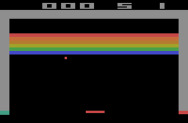
\includegraphics[width=1.0\textwidth]{Static/chap1_robust_atari.jpg}
        \subcaption{Atari game scene\cite{patel2019improved}}
        \label{fig:robust:atari}
    \end{minipage}

    \caption[SNNの頑健性]{
        (a) ガウシアンノイズに対するSNNの頑健性. 
        SNNを用いた識別モデルはノイズ強度の増加による性能の劣化が小さい.
        (b) Atariゲームにおけるブロック崩し.
        SNNを用いた強化学習エージェントは, 画面の一部を隠した際のスコア低下が小さい.
    }
\end{figure}


\section{筋肉留学}
\subsection{一度目の留学}
2006年10月9日(体育の日)に芸能生活を一時休業し、一年間の予定でボディビルダーにとっての聖地であるロサンゼルスへ向かい、自らのトレードマークである肉体を強化するための"筋肉留学"を行った。

2007年2月9日(2月9日の金曜日、筋肉にかけている)カリフォルニア州サンタモニカで全編英語のライブを行った。当初一回公演の予定だったものの現地の観客が多数詰め掛けたため急遽二回公演に変更し、およそ100人ほどの聴衆を前にライブを披露した。現地では「nobody knows your comedic style(前人未踏の芸風)」と評され、「賞賛を得た」と報道されている[6]。キャプテン☆ボンバーも披露し、日本とは逆に日本の文化をネタにしていた。2007年8月31日(現地時間)、初めて自らが主演・監督・脚本を担当した35分の自主製作映画「キャプテン☆ヒーロー」を公開。

2007年9月7日、予定期間を終えて筋肉留学から帰国。帰国した模様が同日に放送の毎日放送『ちちんぷいぷい』で取り上げられた。その翌日には毎日放送『せやねん!』に生出演。帰国後初のテレビ番組出演で、3日後の9月10日には読売テレビ『なるトモ!』にも生出演した。9月29日には『せやねん!』に帰国後2回目の生出演、レギュラー番組に復帰した。2007年のM-1グランプリのために同じく筋肉質の芸人八木真澄(サバンナ)と漫才コンビ「ザ☆健康ボーイズ」を結成し、準決勝進出の好成績を挙げた。2008年も「ザ☆健康ボーイズ」として、M-1に再挑戦[7]しており、現在もそれぞれの活動と並行して不定期でのコンビ活動を継続している[注 5]。同年には日本テレビ『ダウンタウンのガキの使いやあらへんで!!』で筋肉料理研究家マグマ中山として出演し、以降も定期的にこのネタを行っている。

% svgのままぶち込む
\begin{figure}[htbp]
  \centering
  \includesvg[width=0.5\textwidth, inkscapelatex=false]{Chapter1/figures/kinniku}
  \caption{筋肉SVG}
  \label{fig:my_label}
\end{figure}

% Learning Based
\subsection{二度目の留学}
帰国後の芸能活動を順調に再開しつつあった2008年1月23日、「1年間程度では大した成果が出ない」との考えから今度は永住覚悟、あるいは無期限での筋肉留学を開始した。アメリカでは一度目のように肉体強化だけではなく、語学勉強や空手ジムに通うなどの本格的な留学計画を立てている[7]。渡米後、カルフォルニア州の2年制の公立大学であり、アーノルド・シュワルツェネッガーの母校でもあるサンタモニカ・カレッジに留学した。

再留学後も定期的に帰国しており、留学40日後の2008年3月3日にはビザの申請のため急遽帰国し、改めてアメリカに向かっていた[8][9][注 6]。3月27日発売の「モンスターハンターポータブル 2nd G」のCM「芸人編」に起用された他、M-1グランプリへの再挑戦(詳細は前述)のため、10月29日にも一時帰国している。日本滞在中は「LIVE STAND 08 OSAKA」への出演に加え、留学前まで準レギュラーだった『せやねん!』をはじめ、フジテレビ『爆笑レッドカーペット』、TBS『ウンナン極限ネタバトル! ザ・イロモネア 笑わせたら100万円』などにも出演した。同年12月末に再渡米。留学の目的の一つとして「アメリカの映画やコメディショーに出演したい」という夢があり実際オーディションにもいくつか合格していたものの、留学ビザしか取得していなかったため出演は叶わなかったという[10]。

2010年7月、先輩のなだぎ武がブログ上で「留学前より線が細くなった」と写真付きで報告しており[11]、むしろ筋力的にも衰えた状態となっていた。2011年1月、サンタモニカ・カレッジ運動生理学部を卒業した[12]。成績はGPA3.38と好成績を収めており、授業も日常会話も全て英語の環境で真面目に授業を受けていたことが明らかになり、憧れのシュワルツェネッガーの名も正確に発音できる(本人談)レベルの語学力を獲得した。卒業を記念してレイザーラモンHG(レイザーラモン)をゲストに「Muscle Comedy 3 〜筋肉留学卒業公演〜」をキャンパス内で開催した。
\section{先行研究での課題}
先行研究では, SNNにおける時定数をニューラルネットワークの重みとバイアスと同様に学習可能とすることで, SNNの時間表現力を向上させた.
しかしながら, 入力速度に対する汎化性の面で課題があると考えられる.
時定数の学習による時間表現能力の向上には, 学習時に多様な速度帯のデータを与える必要がある.
これは, 速度倍率の変化によって, データのタイムステップ間の時間関係が変化するため, それぞれの速度域に対応可能な時定数を学習する必要があるためである.
しかしながら, このような速度のみが異なるデータは時間的特性以外は類似の情報を持つことが多く, その学習効率が低下する.
例えば, ジェスチャー認識のデータセットでは, 速度の高低に関わらず同一のジェスチャーである.
そのため, 入力速度変化に対して頑健な推論を行うために, 基準速度データの学習のみで汎化性の高いSNNを構築することが望ましいと考えられる.

\section{研究目的}
本研究の目的は, 未学習の入力速度に対して汎化なSpiking Neural Networkを構築することである.
この目的のために, 時定数を含むSNNのパラメータを推論時にも動的に変化させる機構を提案する.
先行研究と提案手法の時定数に対するアプローチの違いを\tabref{tab:method:comparison}に示す.
先行研究では, 時定数は学習可能であったが, 推論時にはその学習済みの時定数を固定して使用する.
本研究では, 時定数が学習可能であることに加えて, 推論時には時定数が動的に変化する.
これによって, 未学習の速度帯のデータであっても, SNNの振る舞いが学習時の速度帯が入力された場合と同様になることが期待される.
結果として, 入力速度帯に関係なく汎化なSNNを構築することが可能となる.
本研究では, 提案手法をSNNに組み込み, その原理の実験的検証と実問題への適用を行う.
\begin{table}[htb]
    \centering
    \caption[先行研究と提案手法の時定数に対するアプローチ比較]{
        先行研究と提案手法の時定数に対するアプローチ比較. 提案手法のみ推論時の時定数が動的に変化する.
    }
    \label{tab:method:comparison}
    %{\small %12ptだとはみ出るので小さく
    \begin{tabular}{cccc}
        \hline
         & \textbf{従来のSNN} & \textbf{先行研究}\cite{dhsnn,paramsnn} & \textbf{提案手法}\\
        \hline
        事前設定 & 固定 & なし & なし\\
        学習時 & 学習不可 & 学習可能 & 学習可能\\
        推論時 & 固定 & 固定 & \textbf{動的}\\
        \hline
    \end{tabular}
    %}
\end{table}

\section{本論文の構成}
本論文の構成は以下に示す通りである.

\subsubsection{第1章 序論}
本研究の背景および先行研究について述べた.
また, 先行研究での課題とその課題に対する本論文の目的を述べた.

\subsubsection{第2章 手法}
本研究で用いるSpiking Neural Networkの生物学的背景とそのモデル化, 学習則について述べる.
また, 本研究の提案手法とその導出過程を記述する.
さらに, 提案手法を用いた実験内容について述べる.

\subsubsection{第3章 実験結果}
未記載

\subsubsection{第4章 考察}
未記載

\subsubsection{第5章 結言}
未記載



\cleardoublepage % 奇数ページから始める
\chapter{手法}
\section{Spiking Neural Network (SNN)}
本節ではまず, Spiking Neural Network (SNN)の生物学的背景について述べる.
その後, Spiking Neural Network (SNN) の基本構成について述べる.

\subsection{生物学的背景}
Spiking Neural Network (SNN)は, 生物の脳神経回路を模倣した数理モデルである.
脳神経回路は, ニューロンと呼ばれる細胞体, 樹状突起, 軸索, シナプスからなる要素の接続によって構成される.
無数のニューロンによって, 入力された電気パルスが出力信号に変換されることで, 生物のような複雑なダイナミクスを表現することが可能となる.

典型的なニューロンの構成要素について\figref{fig:brain:neuron}に示す.
まず, 細胞体は数マイクロメートルから数十マイクロメートルほどの大きさ, 樹状突起の長さは数十マイクロメートルから1ミリメートル程度である.
軸索の長さは長いもので1メートル近くに達する.
ニューロンにおける情報は, 樹状突起から細胞体, 軸索を通してシナプスに向かい, 他のニューロンへと伝達される.
まず樹状突起は, 前に接続されたニューロンのシナプスから信号を受け取る.
この信号によって, 樹状突起や細胞体の中の内部状態である膜電位が変化する.
このとき, 膜電位を正の方向に変化させる信号を興奮性シナプス, 負の方向に変化させる信号を抑制性シナプスと呼ぶ.
興奮性シナプスと抑制性シナプスによる刺激によって, 膜電位があるしきい値を超えると, 膜電位が急激に上昇する.
この電圧は活動電位と呼ばれ, パルス状の信号として軸索上を伝達する (\figref{fig:brain:actionpotential}).
伝達速度は0.5 m/sから100 m/s程度であり, 軸索の種類や太さによって大きく差がある.
軸索の終端に電気信号が到達すると, シナプスから化学伝達物質が分泌され, 接続された樹状突起や細胞体の膜電位を変化させる.
このようなニューロンをネットワーク状に接続し, パルス状の信号を伝達することで, 脳神経回路は複雑な情報処理を行っている.

\begin{figure}[htbp]
    \centering

    \begin{minipage}{0.497\textwidth}
        \centering
        \includesvg[width=1.0\textwidth, inkscapelatex=false]{Static/chap2_sec1_brainneuron}
        \subcaption{神経細胞の構成}
        \label{fig:brain:neuron}
    \end{minipage}
    \hspace{0.02\textwidth}
    \begin{minipage}{0.3474\textwidth}
        \centering
        \includesvg[width=1.0\textwidth, inkscapelatex=false]{Static/chap2_sec1_brainactv}
        \subcaption{膜電位の上昇によるパルス信号の出力}
        \label{fig:brain:actionpotential}
    \end{minipage}

    \caption[脳神経回路の模式図]{
        \cite{lobo2020spiking}
        (a) 神経細胞の構成. 
        樹状突起 (dendrites), 軸索 (axon), シナプス (synapse), 細胞体 (soma) を構成要素として持つ.
        (b) 膜電位の上昇によるパルス信号の出力.
        細胞体の膜電位 (Action Potential) が閾値を超えるとパルス信号が出力される.
    }
\end{figure}
\subsection{Spiking Neural Networkの構成}

Spiking Neural Network (SNN) は前述したニューロンにおけるパルス信号を介した情報処理を模倣したニューラルネットワークである.
そのため, 通常のArtificial Neural Network (ANN) と比較して, より生物的妥当性が高いモデルと考えられている.
SNNはパルス状の電気信号を, スパイクと呼ばれる0か1の値を持つ信号として扱う.
さらに, スパイクが時間軸に沿って並べられたものをスパイク列と呼び, SNNはこのスパイク列をニューロン間で伝達することで, ニューロンの時間的なダイナミクスを模倣し情報処理を行う.

SNNの第$l$層における入出力の流れを\figref{fig:snn:inoutflow}に示す.
まず, SNNへ入力されたスパイク$\bm{o}^{t, l-1}$は\eqrefc{eq:input_spike}によって重み付けされシナプス電流$\bm{i}^{t,l}$へ変換される.

\begin{equation}
    \bm{i}^{t, l} = \bm{W}^l\bm{o}^{t, l-1} + \bm{b}^l
    \label{eq:input_spike}
\end{equation}
ここで, $t$はその時刻を表し, $\bm{W}^l, \bm{b}^l$はそれぞれ第$l$層のニューラルネットワークの重みとバイアスを表す.

次に, 第$l$層のSNNの内部状態$\bm{v}^{t, l}$は, 神経細胞活動の数理モデルによって更新される.
本研究では, 数理モデルとしてLeaky Integrate-and-Fire (LIF) モデル\eqrefc{eq:lif}を用いる.
LIFモデルとは, 入力シナプス電流を, 神経細胞の内部状態があるしきい値に達するまで時間的に積分するモデルである.

\begin{equation}
    {\tau}\frac{d\bm{v}^l}{dt}=-\left(\bm{v}^l\left({t-1}\right)-v_{rest}\right)+r\bm{i}^{t, l}
    \label{eq:lif}
\end{equation}
ここで, $\tau$は神経細胞の時定数, $v_{rest}$は内部状態の初期状態, $r$は神経細胞の膜抵抗である.

最後に, 内部状態$\bm{v}^{t, l}$が一定の閾値$v_{th}$を超えたときに出力スパイク$\bm{o}^{t, l}$が1となって出力される (\eqrefc{eq:outputSpike}).
また, 閾値を超えた内部状態は初期状態へとリセットされる (\eqrefc{eq:outputSpike2}).

\begin{equation}
    \begin{split}
      \bm{o}^{t, l}&=g\left(\bm{v}^{t, l}\right)\\
    where\\
    g\left(x\right)&=\left\{
      \begin{alignedat}{2}
        1 &\:\left(x{\geq}v_{th}\right)\\
        0 &\:\left(x{<}v_{th}\right)
      \end{alignedat}
    \right. 
    \end{split} \label{eq:outputSpike}
  \end{equation}

  \begin{equation}
    \begin{split}
      \bm{v}^{t, l}&=h\left(\bm{v}^{t, l}\right)\\
    where\\
    h\left(x\right)&=\left\{
      \begin{alignedat}{2}
        &v_{rset} &\:\left(x{\geq}v_{th}\right)\\
        &x &\:\left(x{<}v_{th}\right)
      \end{alignedat}
    \right. 
    \end{split} \label{eq:outputSpike2}
  \end{equation}


\begin{figure}[htb]
    \centering
    % \includesvg[width=0.9\textwidth, inkscapelatex=false]{Static/chap2_sec1_snn}
    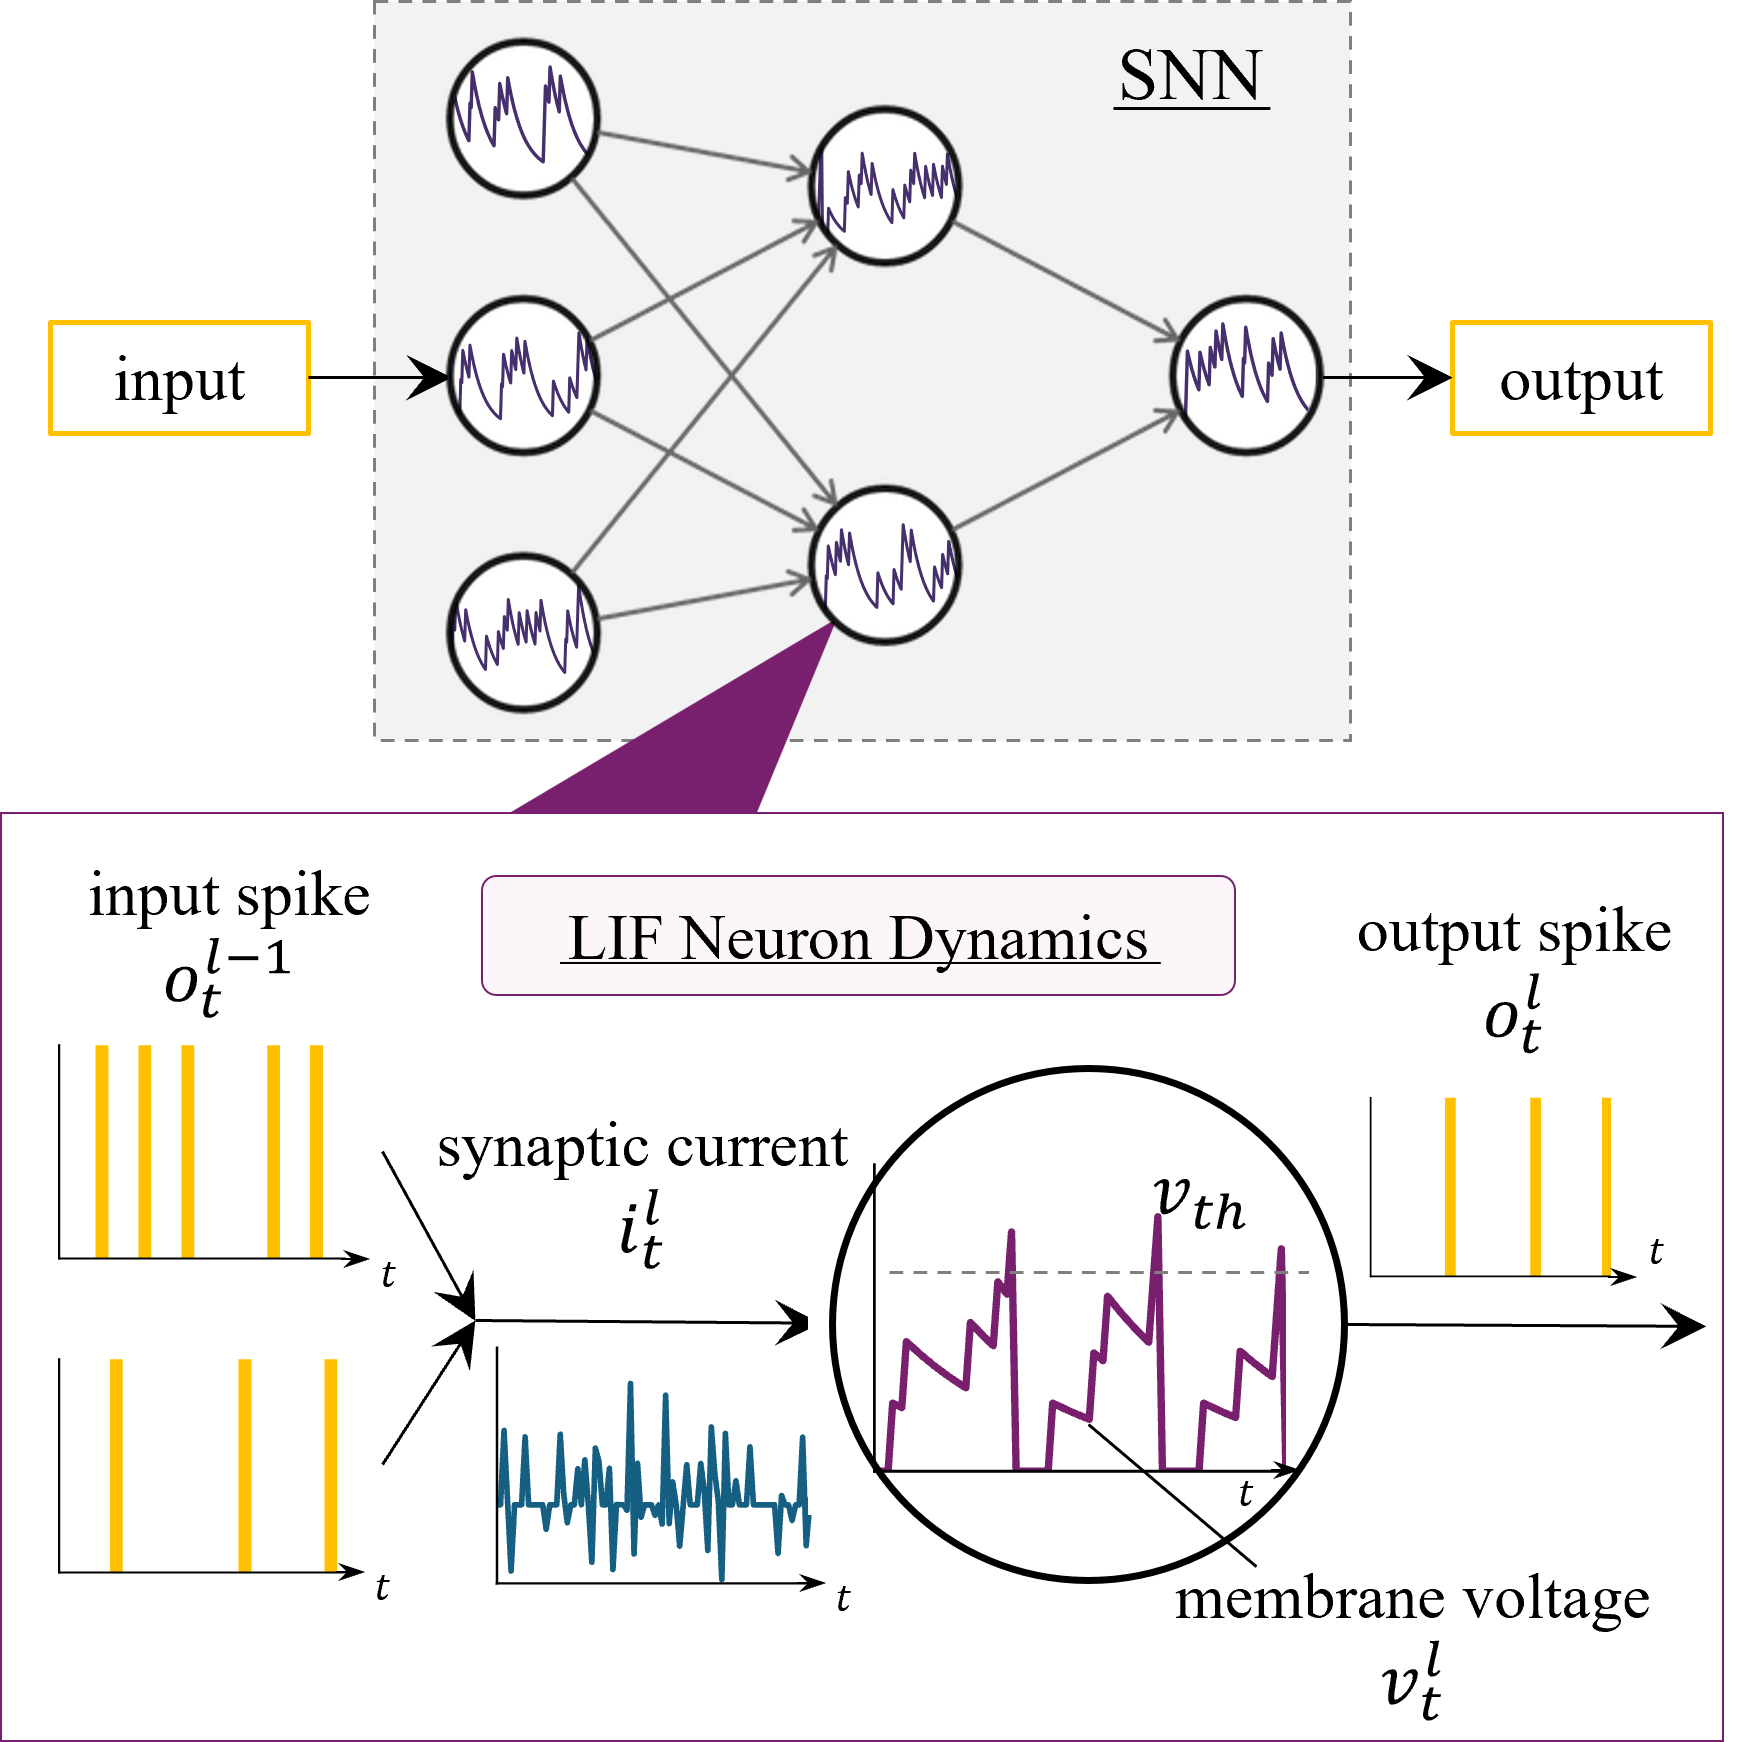
\includegraphics[width=0.75\textwidth]{Static/chap2_sec1_snn.png}
    \caption{SNNの入出力の流れ}
    \label{fig:snn:inoutflow}
\end{figure}

% \subsection{Spatio-Temporal Back Propagation (STBP) によるSpiking Neural Networkの学習}

一般的に, ANNの学習には誤差逆伝播法が用いられる.
誤差逆伝播法とは, ニューラルネットワークの出力と学習データの損失の勾配を用いて, ネットワークの各パラメータを更新する手法である.
本研究では, 誤差逆伝播法をSNNの学習に拡張したSpatio-Temporal Backpropagation (STBP)則\cite{stbp}を用いる.

SNNは時間的に連続なスパイク列を処理するため, 時間的・空間的な情報を同時に扱う.
さらに, スパイクは0か1の不連続な値を持つため, その勾配は消失または発散してしまう.
このため, ANNに用いられる誤差逆伝播法はそのまま用いることができない.
そこで, STBP則では空間情報と時間情報の両方の損失に対して勾配を計算し, さらに, スパイクの勾配を近似関数を用いて表現することで, 近似的に誤差逆伝播法を実現する.

LIFモデルをニューロンモデルとしたSNNに対し, 初期条件$v(t)|_{t=t_{i-1}}=v(t_{i-1})$としたときの\eqrefc{eq:lif}の線形微分方程式の解は\eqrefc{eq:snn:lif:diff}となる.
\begin{equation}
    v(t) = v \left(t_{i-1}\right) \mathrm{e}^{-\frac{t-t_{i-1}}{\tau}} + i(t)
    \label{eq:snn:lif:diff}
\end{equation}
ここで, 簡易のために$r=1$としているが, その一般性は失われない.

ある時刻$t$のニューロン内部状態$v(t)$の値は\eqrefc{eq:snn:lif:diff}により, 入力シナプス電流$i(t)$の空間的な蓄積と, 以前の内部状態$v(t_{i-1})$の記憶量によって決定される.
そこで, \eqrefc{eq:snn:lif:diff}で得られた解を用いて, ニューロンの内部状態とその入出力は以下のように記述できる(\eqrefc{eq:snn:lif:state},\eqrefc{eq:snn:lif:state2},\eqrefc{eq:snn:lif:state3}).

\begin{align}
    x_i^{t+1,l} &= \sum_{j=1}^{N(l-1)} w_{ij}^{l} o_j^{t+1,l-1} \label{eq:snn:lif:state} \\
    v_i^{t+1,l} &= v_i^{t,l} f\left(o_i^{t,l}\right) + x_i^{t+1,l} + b_i^l \label{eq:snn:lif:state2} \\
    o_i^{t+1,l} &= g\left(v_i^{t+1,l}\right) \label{eq:snn:lif:state3}\\
    where\\
    f\left(x\right) &= \tau \mathrm{e}^{-\frac{x}{\tau}} \label{eq:snn:lif:state4}
\end{align}


ここで, $w_ij$は第$l$層の$i$番目のニューロンと第$l-1$層の$j$番目のニューロンの間のシナプス結合の重み, $b_i^l$は第$l$層の$i$番目のニューロンのバイアスである.
また, $o_j$は0または1の値を持ち, ニューロンの発火スパイクを表す.
$N(l)$は第$l$層のニューロン数に対応する.
\eqrefc{eq:snn:lif:state2}はニューロン内部状態の時間変化を表しており, 1項目の$v_i^{t,l} f\left(o_i^{t,l}\right)$は過去の内部状態の記憶, 2項目と3項目の$x_i^{t+1,l}$と$b_i^l$は現在の入力を表す.

STBPにおける時間的・空間的な損失勾配の概要を\figref{fig:snn:stbp:single}と\figref{fig:snn:stbp:network}に示す. 
\figref{fig:snn:stbp:single}は単一のニューロン, \figref{fig:snn:stbp:network}はネットワークにおける勾配の伝播を表す.
STBPは空間的な勾配と時間的な勾配を伝播することで, ネットワークのパラメータを更新する.
空間的な勾配は, 通常のニューラルネットワークにおける誤差逆伝播法と同様に, 出力の損失勾配から重みとバイアスの勾配を計算する.
一方, 時間的な勾配は, Recurrent Neural Network (RNN) における誤差逆伝播法である Backpropagation Through Time (BPTT) と同様に, 時間的な損失勾配からニューロンの内部状態の勾配を計算する.
\begin{figure}[htbp]
    \centering

    \begin{minipage}{0.45\textwidth}
        \centering
        \includesvg[width=1.0\textwidth, inkscapelatex=false]{Static/chap2_sec1_stbp1}
        \subcaption{単一ニューロンの勾配}
        \label{fig:snn:stbp:single}
    \end{minipage}
    \hspace{0.02\textwidth}
    \begin{minipage}{0.45\textwidth}
        \centering
        \includesvg[width=1.0\textwidth, inkscapelatex=false]{Static/chap2_sec1_stbp2}
        \subcaption{ネットワークの勾配}
        \label{fig:snn:stbp:network}
    \end{minipage}

    \caption[STBP則における時間的・空間的な損失勾配の概要]{
        \cite{stbp}
        (a) 単一ニューロンの勾配.
        $SD, TD$はそれぞれ空間的, 時間的な損失勾配を表す.
        (b) ネットワークの勾配.
    }
\end{figure}


STBP則における損失関数$L$を\eqrefc{eq:snn:stbp:loss}に示す.
\begin{equation}
    L = \frac{1}{2S} \sum_{s=1}^{S} \left(\bm{y}_s - \frac{1}{T}\sum_{t=1}^{T} \bm{o}_s^{t,L}\right)^2 \label{eq:snn:stbp:loss}
\end{equation}
ここで, $\bm{y}_s, \bm{o}_s^{t,l}$はそれぞれ$s$番目のサンプルにおける教師データとSNNの出力を表す.
また, $\frac{1}{T}\sum_{t=1}^{T} \bm{o}_s^{t,L}$は, 単位時間当たりのスパイクの密度を表す.
STBP則では, 教師データとSNNの単位時間当たりのスパイク密度の損失が小さくなるように, ニューラルネットワークの重みとバイアスを更新する.


STBP則におけるニューラルネットワークの重み$\bm{W}$とバイアス$b$損失勾配は以下のように表される.
\begin{align}
    \frac{\partial L}{\partial \bm{b}^l}
    = \sum_{t=1}^{T} \frac{\partial L}{\partial \bm{v}^{t,l}} \frac{\partial \bm{v}^{t,l}}{\partial \bm{b}^l}
    = \sum_{t=1}^{T} \frac{\partial L}{\partial \bm{v}^{t,l}} \label{eq:stbp:b}
\end{align}

\begin{align}
    \frac{\partial L}{\partial \bm{W}^{l}}
    &= \sum_{t=1}^{T} \frac{\partial L}{\partial \bm{v}^{t,l}} \frac{\partial \bm{v}^{t,l}}{\partial \bm{W}^{l}} \notag \\
    &= \sum_{t=1}^{T} \frac{\partial L}{\partial \bm{v}^{t,l}}  \frac{\partial \bm{v}^{t,l}} {\partial \bm{x}^{t,l}} \frac{\partial \bm{x}^{t,l}}{\partial \bm{W}^{l}} 
    = \sum_{t=1}^{T} \frac{\partial L}{\partial \bm{v}^{t,l}} \bm{o}^{t,l-1 \top} \label{eq:stbp:w}
\end{align}
ここで, $\bm{o}^{t,l-1 \top}$は$t$時刻における第$l-1$層の出力の転置ベクトルを表す.
\eqrefc{eq:stbp:b}と\eqrefc{eq:stbp:w}より, ニューラルネットワークの重み$\bm{W}$とバイアス$b$の勾配は, 損失関数$L$に対する内部状態$\bm{v}$の勾配$\partial L / \partial \bm{v}^{t,l}$によって計算できる.


次に$\partial L / \partial \bm{v}^{t,l}$を求めるが, これは以下の4つのパターンによって場合分けして計算することができる.
ここで, $t$は時刻でありその範囲は$t \in \left[1, T\right]$, $l$はニューラルネットワークの層数でありその範囲は$l \in \left[1, L\right]$と定義される.
また, 表記の簡易化のために損失関数$L$のスパイク$o_i^{t,l}$に対する勾配を$\delta_i^{t,l}$と表す (\eqrefc{eq:stbp:delta}).
\begin{equation}
    \delta_i^{t,l} = \frac{\partial L}{\partial o_i^{t,l}} \label{eq:stbp:delta}
\end{equation}

$t=T, l=L$の場合
\begin{equation}
    \frac{\partial L}{\partial o_i^{T,L}}  = - \frac{1}{TS} (y_i -\frac{1}{T}\sum_{k=1}^{T} o_i^{k,L})
\end{equation}

\begin{equation}
    \frac{\partial L}{\partial v_i^{T,L}} 
    = \frac{\partial L}{\partial o_i^{T,L}} \frac{\partial o_i^{T,L}}{\partial v_i^{T,L}} 
    = \delta_i^{T,L} \frac{\partial o_i^{T,L}}{\partial v_i^{T,L}} \label{eq:stbp:v:case1}
\end{equation}

$t=T, l<L$の場合
\begin{equation}
    \frac{\partial L}{\partial o_i^{T,l}} 
    = \sum_{j=1}^{N(l+1)} \delta_j^{T,l+1} \frac{\partial o_j^{T,l+1}}{\partial o_i^{T,l}} 
    = \sum_{j=1}^{N(l+1)} \delta_j^{T,l+1} \frac{\partial g}{\partial v_i^{T, l}} w_{ji}
\end{equation}

\begin{equation}
    \frac{\partial L}{\partial v_i^{T,l}} 
    = \frac{\partial L}{\partial o_i^{T,l}} \frac{\partial o_i^{T,l}}{\partial v_i^{T,l}} 
    = \delta_i^{T,l} \frac{\partial g}{\partial v_i^{T,l}} \label{eq:stbp:v:case2}
\end{equation}

$t<T, l=L$の場合
\begin{align}
    \frac{\partial L}{\partial o_i^{t,L}} 
    &= \delta_i^{t+1,L} \frac{\partial o_j^{t+1,L}}{\partial o_i^{t,L}} + \frac {\partial L} {\partial o_i^{t,L}} \notag \\ 
    &= \delta_i^{t+1,L} \frac{\partial g}{\partial v_i^{t+1,L}} v_i^{t,L} \frac{\partial f}{\partial o_j^{t,L}} + \frac {\partial L} {\partial o_i^{t,L}}
\end{align}

\begin{align}
    \frac{\partial L}{\partial v_i^{t,L}} 
    = \frac {\partial L} {\partial v_i^{t+1,L}} \frac {\partial v_i^{t+1,L}} {\partial v_i^{t,L}} 
    = \delta_i^{t+1,L} \frac {\partial g} {\partial v_i^{t+1,L}} f(o_i^{t,L}) \label{eq:stbp:v:case3}
\end{align}

$t<T, l<L$の場合
\begin{align}
    \frac{\partial L}{\partial o_i^{t,l}} 
    &= \sum_{j=1}^{N(l+1)} \delta_j^{t,l+1} \frac{\partial o_j^{t,l+1}}{\partial o_i^{t,l}} + \frac {\partial L} {\partial o_i^{t+1,l}} \frac{\partial o_i^{t+1,l}}{\partial o_i^{t,l}}  \notag \\
    &= \sum_{j=1}^{N(l+1)} \delta_j^{t,l+1} \frac{\partial g}{\partial v_i^{t,l}} w_{ji} 
    + \delta_i^{t+1,l} \frac{\partial g}{\partial v_i^{t,l}} v_i^{t,l} \frac{\partial f}{\partial o_i^{t,l}}
\end{align}         

\begin{align}
    \frac{\partial L}{\partial v_i^{t,l}} 
    &= \frac {\partial L} {\partial o_i^{t,l}} \frac {\partial o_i^{t,l}} {\partial v_i^{t,l}} + \frac {\partial L} {\partial o_i^{t+1,l}} \frac {\partial o_i^{t+1,l}} {\partial v_i^{t,l}} \notag \\
    &= \delta_i^{t,l} \frac {\partial g} {\partial v_i^{t,l}} 
    + \delta_i^{t+1,l} \frac {\partial g} {\partial v_i^{t+1,l}} f(o_i^{t,l}) \label{eq:stbp:v:case4}
\end{align}


ここで, $g(v)$は0か1のスパイクを出力する関数であり, その勾配$\partial g / \partial v$は消失または爆発してしまう.
そのため, 上記の4つ場合における$\partial L / \partial \bm{v}^{t,l}$の値をそのまま用いて, 重みとバイアスの勾配を計算してもネットワークの学習は進行しない.
そこで, $\partial g / \partial v$を近似関数で表すことでネットワークの学習を進行させる.
近似関数を\eqrefc{eq:stbp:g1} - \eqrefc{eq:stbp:g4}に示す.
\begin{equation}
    \frac{\partial g}{\partial v} = \frac{1}{a_1} \, \text{sign}\left(|v - v_{th}| < \frac{a_1}{2}\right) \label{eq:stbp:g1}
\end{equation}

\begin{equation}
    \frac{\partial g}{\partial v} = \left(\frac{\sqrt{a_2}}{2} - \frac{a_2}{4} |v - v_{th}|\right) \text{sign}\left(\frac{2}{\sqrt{a_2}} - |v - v_{th}|\right) \label{eq:stbp:g2}
\end{equation}

\begin{equation}
    \frac{\partial g}{\partial v} = \frac{1}{a_3} \frac{ \mathrm{e}^{\frac{v_{th}-v}{a_3} }} {\left( 
        1 + \mathrm{e}^{\frac{v_{th}-v}{a_3}}
     \right)^2} \label{eq:stbp:g3}
\end{equation}

\begin{equation}
    \frac{\partial g}{\partial v} = \frac{1}{\sqrt{2\pi a_4}} e^{-\frac{\left(v - v_{th}\right)^2}{2a_4}} \label{eq:stbp:g4}
\end{equation}

ここで, sign関数は入力の符号に応じて, $1, -1, 0$のいずれかを出力する関数である(\eqrefc{eq:stbp:sign}).
\begin{equation}
    \text{sign}(x) = \begin{cases}
        1 & (x > 0) \\
        -1 & (x < 0) \\
        0 & (x = 0)
    \end{cases} \label{eq:stbp:sign}
\end{equation}
また, $a_i$は各関数の積分が1になるような定数である.
それぞれの導関数の外形図を\figref{fig:snn:stbp:pesudo:grad}に示す.
導関数は釣鐘状の形状をしており, ディラックのデルタ関数を近似している.
これらの近似関数はどの形状であっても, その学習精度は大きく変動しないことが知られている.
本研究では, \eqrefc{eq:stbp:g3}のfast sigmoid関数を用いることでSTBP則での学習を行った.

以上よりSTBP則では, 内部状態の勾配\eqrefc{eq:stbp:v:case1} - \eqrefc{eq:stbp:v:case4}と導関数の近似を用いることで, 時空間方向に対して重み$\bm{W}$とバイアス$\bm{b}$を\eqrefc{eq:stbp:b}と\eqrefc{eq:stbp:w}によって学習することが可能となる.

\begin{figure}[htbp]
    \centering

    \begin{minipage}{0.45\textwidth}
        \centering
        \includesvg[width=1.0\textwidth, inkscapelatex=false]{Static/chap2_sec1_pesudo1}
        \subcaption{スパイク出力関数$g(v)$とその勾配}
        \label{fig:snn:stbp:g}
    \end{minipage}
    \hspace{0.02\textwidth}
    \begin{minipage}{0.45\textwidth}
        \centering
        \includesvg[width=1.0\textwidth, inkscapelatex=false]{Static/chap2_sec1_pesudo2}
        \subcaption{$\frac{dg}{dv}$の近似関数}
        \label{fig:snn:stbp:pesudo:grad}
    \end{minipage}

    \caption[スパイク出力関数の勾配の近似関数]{
        \cite{stbp}
        (a) スパイク出力関数$g(v)$とその勾配. 
        勾配${dg}/{dv}$はディラックのデルタ関数$\delta(v)$で表現される.
        (b) ${dg}/{dv}$の近似関数.
        $h_1, h_2, h_3, h_4$はそれぞれ\eqrefc{eq:stbp:g1} - \eqrefc{eq:stbp:g4}の近似関数を表す.
    }
\end{figure}

\section{提案手法}
本節ではまず, 提案手法の概要について述べる.
その後, 提案手法である入力速度変化に対して頑健なSNNの定式化を行う.

\subsection{提案手法 概要}
提案手法の概要図を\figref{fig:proposed_method}に示す.
本手法では, 入力スパイク列$\bm{o}(t)$の未学習の速度に対して, その推論精度が低下しにくいSNNを実現することを目指す.
一般的に, ニューラルネットワークは入力の加減速に対して, その内部状態は単純な加減速とはならない.
そのため, ニューラルネットワークの最終的な出力は, 入力の速度変化に依存して変化する.
そこで本手法では, 入力の速度変化に応じて, SNNの内部状態の変化量を動的に調整する機構を導入する.
内部状態の変化量の調整は, 時定数$\tau$を含むSNNのパラメータ (\figref{fig:proposed_method}における$\tau', r'$) を推定器で推定し, その推定値を適用することで行う.
この機構によって, 入力速度変化による内部状態の変化を抑制し, 頑健な推論を行うSNNを構築する.

\begin{figure}[htb]
    \centering
    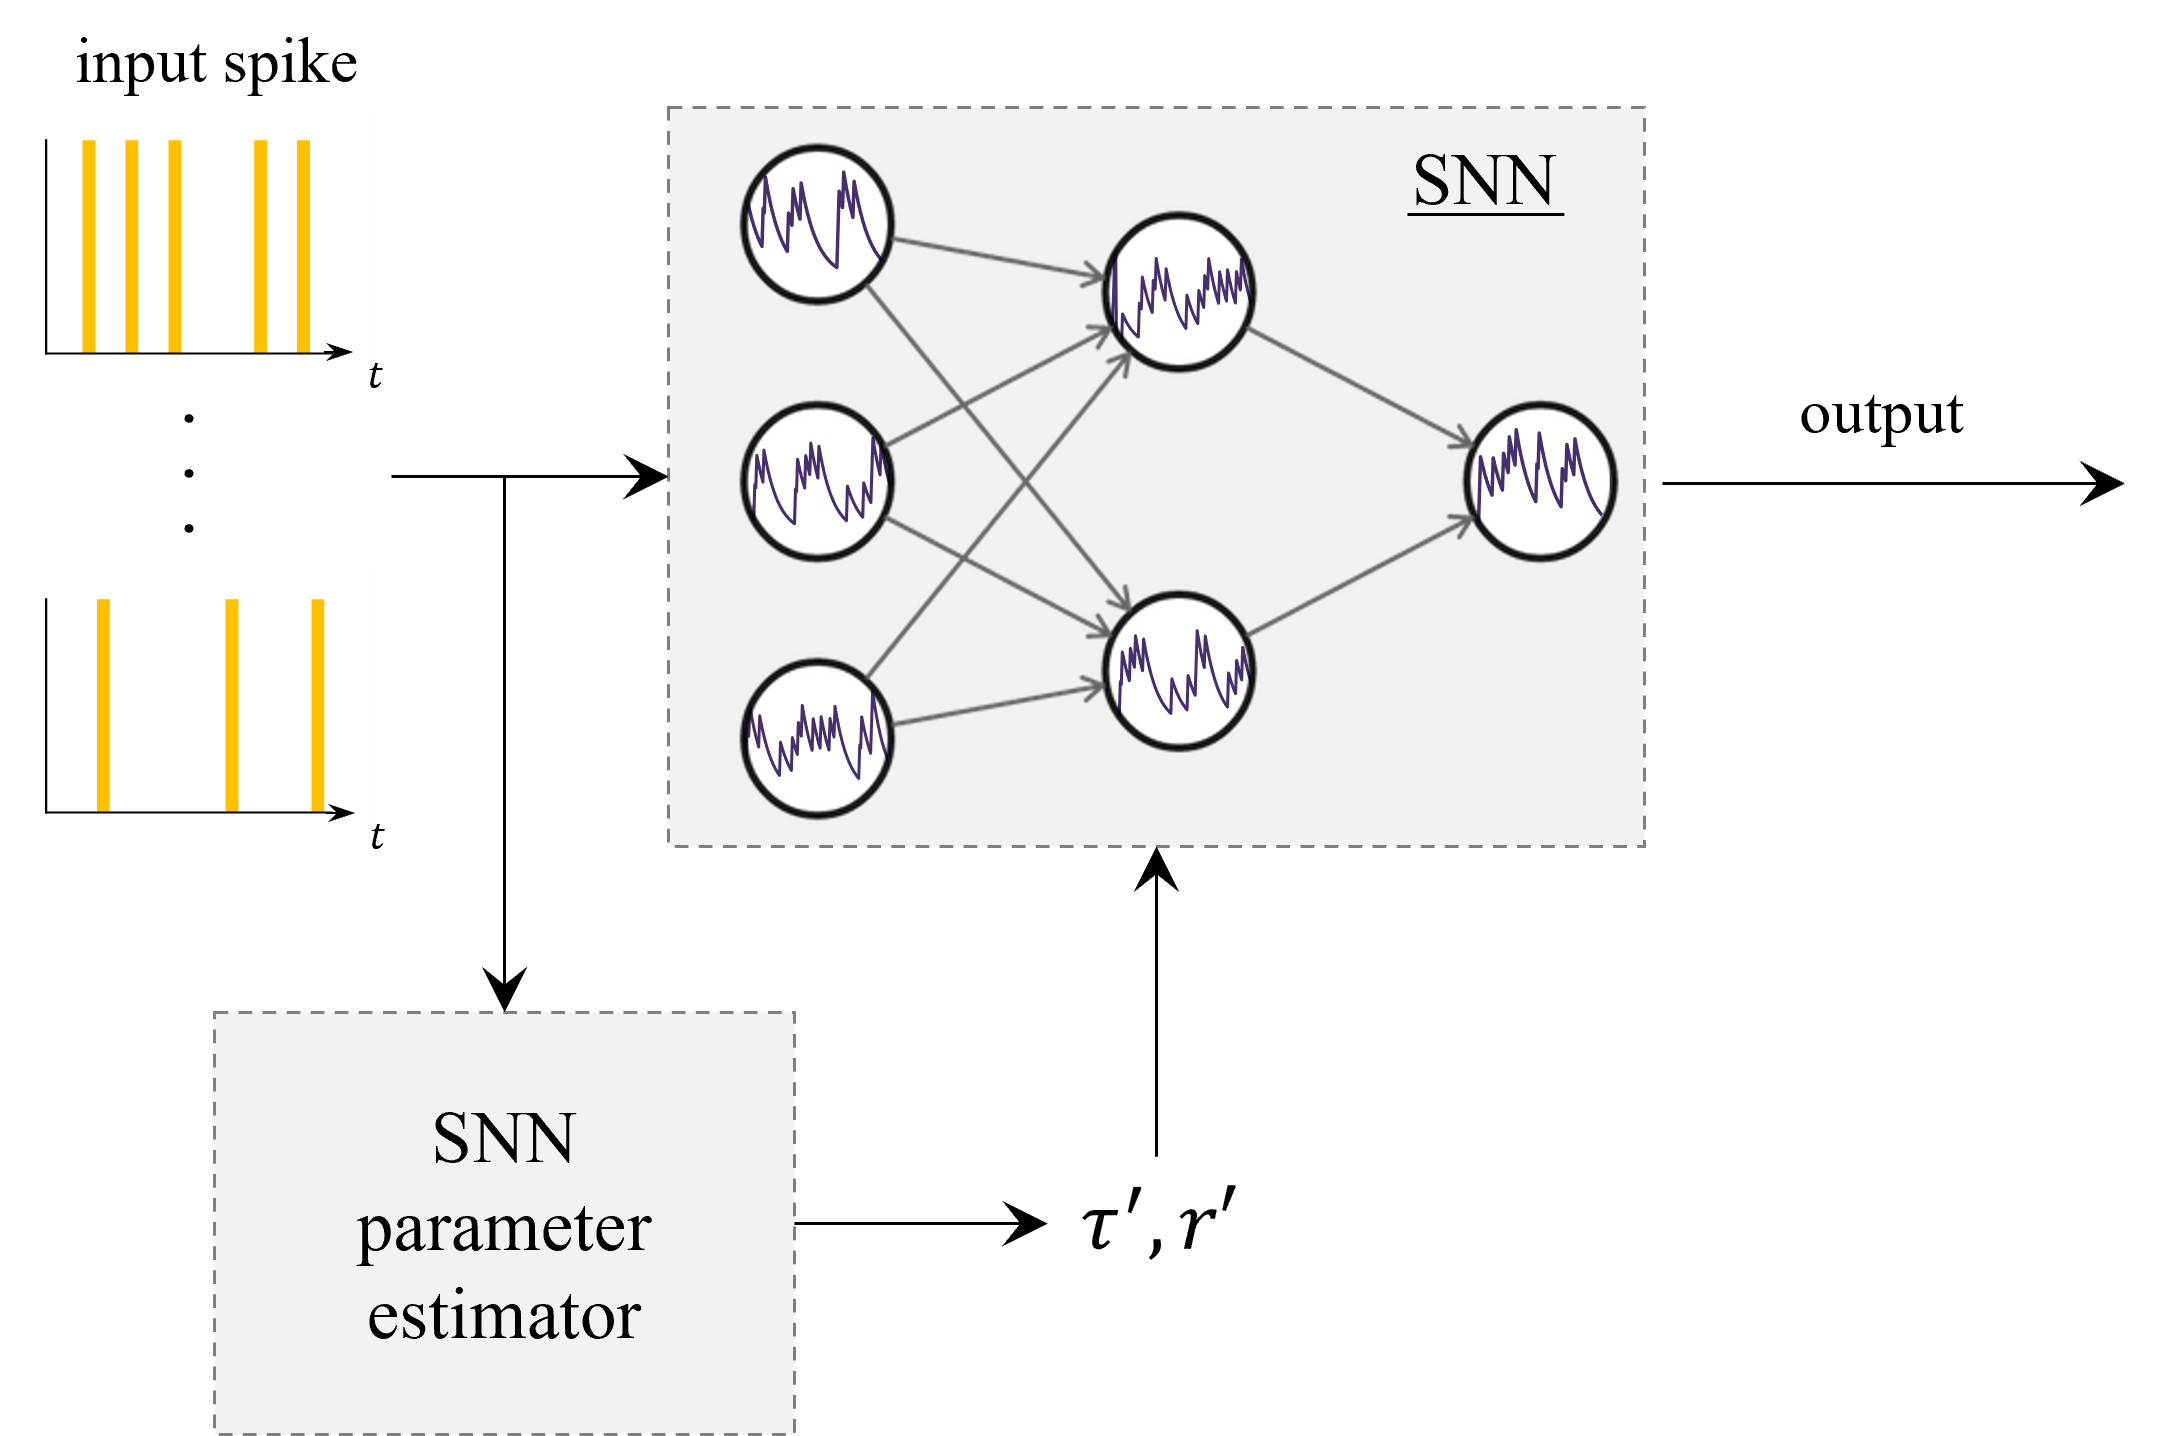
\includegraphics[width=0.9\textwidth]{Static/chap2_sec2_methodstr.png}
    \caption[提案手法の概要図]{
        提案手法の概要図.
        $\tau', r'$はそれぞれ時定数$\tau$と膜抵抗$r$の推定値を表す.
    }
    \label{fig:proposed_method}
\end{figure}

提案手法の導出は以下の3ステップで行う.
\begin{enumerate}
    \item 入力スパイク列の速度変化に対する理想的なSNNの内部状態の定式化
    \item 入力スパイク列の速度変化に対する実際のSNNの内部状態の定式化
    \item 実際の内部状態を理想的な内部状態に近似するための条件の導出
\end{enumerate}
ここで, 理想的なSNNの内部状態とは, 入力スパイク速度が$a$倍になった場合に, 内部状態の変化速度も$a$倍になることを意味する.
実際の内部状態を理想的な内部状態に近似できる条件を導出 (\figref{fig:proposed_method_intro}) し, その条件を満たすようにSNNの時定数および膜抵抗の値を推定することで, 入力速度変化による内部状態の変化を抑制する.
\begin{figure}[htb]
    \centering
    \includesvg[width=0.9\textwidth, inkscapelatex=false]{Static/chap2_sec2_methodintro}
    \caption[提案手法の導出の概要図]{
        提案手法の導出の概要図.
        $v(at), v(t)$はそれぞれ理想的なSNNの内部状態と実際のSNNの内部状態を表す.
    }
    \label{fig:proposed_method_intro}
\end{figure}



\subsection{SNN内部状態近似式の導出} \label{method:proposed}

\subsubsection{入力スパイク列の速度変化に対する理想的なSNNの内部状態の定式化}
本手法では, 入力速度変化に対してSNNの内部状態変化が依存しない状態を理想的と考える.
そのため, 入力スパイク$o(t)$の$a$倍のタイムスケーリングに対して, SNNの内部状態$v(t)$も同様に$a$倍のタイムスケーリングになることが望ましい.
ここで, $a$倍のタイムスケーリングとは, 時刻$t_i$における値が時刻$at_i$における値に時間シフトすることを意味する.
LIFモデル (\eqrefc{eq:lif}) を用いて, 理想状態における入力スパイク$o(t)$と内部状態$v(t)$を表すと\eqrefc{eq:ideal:state}となる.
\begin{align}
    \tau \frac{dv\left(at\right)}{dt} &= -\left(v\left(at\right) - v_{rest}\right) + r i\left(at\right) \notag \\
     &= -\left(v\left(at\right) - v_{rest}\right) + r \left( wo\left(at\right) + b \right) \label{eq:ideal:state}
\end{align}
ここで, 簡易化のためにSNNにおける, ある1ニューロンについてのみを考える.
$o(at), v(at)$はそれぞれ$a$倍のタイムスケーリングを行った入力スパイクとSNNの内部状態を表す.
また, $r, \tau$はそれぞれ理想状態における膜抵抗と時定数を表す.

次に, ラプラス変換を用いて\eqrefc{eq:ideal:state}を$s$領域に変換すると\eqrefc{eq:ideal:state:laplace}と表される.
\begin{align}
    \tau \frac{s}{a} V\left(\frac{s}{a}\right) &= -\left(\frac{1}{a} V\left(\frac{s}{a}\right) 
    - \frac{v_{rest}}{s}\right) + r \left( \frac{w}{a} O\left(\frac{s}{a}\right) + \frac{b}{s} \right) \notag \\
    \left(\tau s +1\right) V\left(\frac{s}{a}\right)  &= \frac{a}{s} v_{rest} +ar \left( \frac{w}{a} O\left(\frac{s}{a}\right) + \frac{b}{s} \right) \notag \\
    V\left(\frac{s}{a}\right) &=  \frac{1}{\tau s +1}\left( \frac{a}{s} v_{rest} +rw O\left(\frac{s}{a}\right) + \frac{a}{s}rb \right) \label{eq:ideal:state:laplace}
\end{align}
ここで, $V(s), O(s)$はそれぞれSNNの内部状態$v(t)$と入力スパイク$o(t)$のラプラス変換を表す.


\subsubsection{入力スパイク列の速度変化に対する実際のSNNの内部状態の定式化}
次に, 入力スパイク列の速度変化が生じたときの実際のSNNの内部状態を定式化する.
入力スパイク$o(t)$に対して$a$倍のタイムスケーリングが生じた場合, 実際の内部状態$v(t)$は単純なタイムスケーリングが生じるとは限らない.
そのため, このときの入力スパイク$o(t)$と内部状態$v(t)$をLIFモデルを用いて表すと\eqrefc{eq:actual:state}となる.
\begin{align}
    \tau_{actual} \frac{dv\left(t\right)}{dt} &= -\left(v\left(t\right) - v_{rest}\right) + r_{actual} i\left(at\right) \notag \\
     &= -\left(v\left(t\right) - v_{rest}\right) + r_{actual} \left( wo\left(at\right) + b \right) \label{eq:actual:state}
\end{align}
% 理想状態における定式化 (\eqrefc{eq:ideal:state}) では, 入力スパイク$o(t)$と内部状態$v(t)$がどちらもタイムスケーリングされていた.
ここで, 入力スパイク$o(t)$のみタイムスケーリングを行い, 内部状態はタイムスケーリングが生じないと仮定している.
そのため, \eqrefc{eq:actual:state}の入力スパイクは$o(at)$となり, 内部状態は$v(t)$となる.
また, $\tau_{actual}, r_{actual}$はそれぞれ実際のSNNの時定数と膜抵抗を表す.

次に, 理想的なSNNの内部状態の定式化 (\eqrefc{eq:ideal:state:laplace}) と同様に, ラプラス変換を用いて\eqrefc{eq:actual:state}を$s$領域に変換すると\eqrefc{eq:actual:state:laplace}と表される.
\begin{align}
    \tau_{actual} sV(s) &= - \left( V(s) - \frac{v_{rest}}{s} \right) + r_{actual} \left( \frac{w}{a} O\left(\frac{s}{a}\right) + \frac{b}{s} \right) \notag \\
    \left(\tau_{actual} s +1\right) V(s) &= \frac{1}{s} v_{rest} +r_{actual} \left( \frac{w}{a} O\left(\frac{s}{a}\right) + \frac{b}{s} \right) \notag \\
    V(s) &=  \frac{1}{\tau_{actual} s +1}\left( \frac{1}{s} v_{rest} +\frac{1}{a} r_{actual} w O\left(\frac{s}{a}\right) + \frac{1}{s} r_{actual} b \right) \label{eq:actual:state:laplace}
\end{align}

さらに, \eqrefc{eq:actual:state:laplace}における$s$を$s/a$に置き換えると, \eqrefc{eq:actual:state:laplace2}が得られる.
\begin{align}
    V\left(\frac{s}{a}\right) &=  \frac{1}{\tau_{actual} \frac{s}{a} +1}\left( \frac{a}{s} v_{rest} +\frac{1}{a} r_{actual} w O\left(\frac{s}{a^2}\right) + \frac{a}{s} r_{actual} b \right) \label{eq:actual:state:laplace2}
\end{align}


\subsubsection{実際の内部状態を理想的な内部状態に近似するための条件の導出}
実際の内部状態における式 (\eqrefc{eq:actual:state:laplace2}) と理想的な内部状態における式 (\eqrefc{eq:ideal:state:laplace}) を比較すると, その近似条件は\eqrefc{eq:approximation:condition1} - \eqrefc{eq:approximation:condition3}で表される3つの式として得られる.
\begin{equation}
    \frac{1}{\tau_{actual} \frac{s}{a} +1} = \frac{1}{\tau s +1}  \label{eq:approximation:condition1}
\end{equation}
\begin{equation}
    \frac{1}{a} r_{actual} w O\left(\frac{s}{a}\right) = r w O\left(\frac{s}{a^2}\right) \label{eq:approximation:condition2}
\end{equation}
\begin{equation}
    \frac{a}{s} r_{actual} b = \frac{a}{s} r b \label{eq:approximation:condition3}
\end{equation}

まず, \eqrefc{eq:approximation:condition1}については, 式変形より\eqrefc{eq:approximation:condition1:result}が得られる.
\begin{align}
    \tau_{actual} = a \tau \label{eq:approximation:condition1:result}
\end{align}

次に, \eqrefc{eq:approximation:condition2}について考える.
$O(s/a), O(s/a^2)$は入力スパイク$o(t)$のラプラス変換である.
ここで, 入力スパイク$o(t)$はディラックのデルタ関数$\delta(t)$として表現される\cite{diracdelta}.
ディラックのデルタ関数$\delta(t)$のラプラス変換は1であるため, $O(s/a) \simeq O(s/a^2) \simeq 1$と近似する.
この近似によって, \eqrefc{eq:approximation:condition2}から\eqrefc{eq:approximation:condition2:result}で表される条件が得られる.
\begin{align}
    \frac{1}{a} r_{actual} w = r w \notag \\
    r_{actual} = a r \label{eq:approximation:condition2:result}
\end{align}

最後に, \eqrefc{eq:approximation:condition3}について考える.
条件\eqrefc{eq:approximation:condition2:result}を用いると, \eqrefc{eq:approximation:condition3}における等式を成り立たせるためには$b=0$とする必要がある.

以上より, 提案手法における条件をまとめると\eqrefc{eq:approximation:condition1:result} - \eqrefc{eq:approximation:condition3:result}で表される3つの式となる.
\begin{align}
    \tau_{actual} &= a \tau \label{eq:approximation:condition1:result} \\
    r_{actual} &= a r \label{eq:approximation:condition2:result} \\
    b &= 0 \label{eq:approximation:condition3:result}
\end{align}
\eqrefc{eq:approximation:condition1:result}は定性的に考えると, 入力速度が低速になった場合はSNNの内部状態の単位時間あたりの変化量を小さくすることを表す.
入力速度が高速になった場合はその逆である.
また, \eqrefc{eq:approximation:condition2:result}は, 入力速度変化によらず入力スパイクの内部状態への影響を一定に保つことを表す.

提案手法では, まずSNNをバイアス0のニューラルネットワークで構成し学習を行う.
推論時には, 入力速度の$a$倍のタイムスケーリングに対して, 時定数$\tau$と膜抵抗$r$をそれぞれ$a$倍することで, その内部状態を単純なタイムスケーリングに近似する.
結果として, 入力速度によらない頑健な推論が可能になると考えられる.

\subsection{入力速度倍率の推定}
提案手法における条件\eqrefc{eq:approximation:condition1:result} - \eqrefc{eq:approximation:condition3:result}では, 入力速度倍率$a$を推定する必要がある.
ここでは, 本手法における入力速度倍率の推定方法について述べる.

まず, 入力速度倍率$a$は, 時刻$t$における入力スパイク$o(t)$が速度変化によって時刻$at$に移動することに対応する (\figref{fig:inspike:scaled}).
次に, 入力スパイク密度$fr$を定義する.
入力スパイク密度$fr$とは, 単位時間当たりのスパイクの数を表す (\eqrefc{eq:input:spike:density}, \figref{fig:firingrate}).
\begin{align}
    fr = \frac{1}{T} \sum_{t=1}^{T} o(t) \label{eq:input:spike:density}
\end{align}
ここで, $T$は時系列データの長さである.
また, 入力速度変化によってその時系列データの情報量 (=スパイクの総数) は変化しないと仮定する.
このことから, 入力速度倍率$a$は, 学習時の基準入力スパイク密度$fr_{base}$と推論時の入力スパイク密度$fr_{in}$の比として推定することができる.
\begin{align}
    a = \frac{fr_{base}}{fr_{in}}
\end{align}

\begin{figure}[htb]
    \centering

    \begin{minipage}{0.9\textwidth}
        \centering
        \includesvg[width=1.0\textwidth, inkscapelatex=false]{Static/chap2_sec3_inspikescale}
        \subcaption{入力スパイクの速度倍率変化}
        \label{fig:inspike:scaled}
    \end{minipage}

    \begin{minipage}{0.5\textwidth}
        \centering
        \includesvg[width=1.0\textwidth, inkscapelatex=false]{Static/chap2_sec3_firingrate}
        \subcaption{スパイク密度$fr$}
        \label{fig:firingrate}
    \end{minipage}

    \caption[入力スパイクの速度倍率変化とスパイク密度]{
        (a) 入力スパイクの速度倍率変化.
        $o(t), o(at)$はそれぞれ元の入力スパイク, 速度倍率変化後のスパイクを表す. 
        (b) スパイク密度$fr$.
    }
\end{figure}



\cleardoublepage % 奇数ページから始める
\chapter{結果}
\section{結果1 入力速度変化に対する内部状態変化の検証結果} \label{sec:result1}
入力スパイクのタイムスケーリングに対して, 本手法を用いることで, SNNの内部状態をタイムスケーリングに近似可能であることを実験的に示す.
本節では, 入力速度変化に対する内部状態変化の結果を定量的, 定性的に示す.

\subsection{入力速度変化に対する内部状態変化の定量評価}
各ネットワーク構造 (\tabref{tab:model:parameter:linear} - \tabref{tab:model:parameter:resnet}) における入力速度変化に対する内部状態変化の結果を\figref{fig:result1:1:linear} - \figref{fig:result1:1:resnet} に示す.
横軸$a$は入力スパイクのタイムスケール倍率, 縦軸は$a=1.0$のときの内部状態と各タイムスケール倍率$a$に置ける内部状態とのMSEを表す.
ここで, タイムスケール$a$は値が小さいほど入力スパイクの速度が速く, 値が大きいほどその速度が遅いことを表す.
また, 青色の破線が通常のSNN, 黄緑色の実線が本手法を用いたSNNを表す.

\figref{fig:result1:1:linear}, \figref{fig:result1:1:cnn}, \figref{fig:result1:1:cnn:dropout}, \figref{fig:result1:1:resnet}より, Linear, CNN, CNN+Dropout, ResNet構造は, 各タイムスケール$a$におけるMSEが小さい値を示した.
特に, タイムスケール$a$が$1.0$よりも大きく, 入力速度が低速化する場合において, 提案手法のMSEが通常のSNNのMSEよりも小さい値を示した.
一方で, \figref{fig:result1:1:cnn:batchnormalization}より, CNN + BatchNormalization構造は提案手法の各タイムスケール$a$におけるMSEが通常のSNNのMSEよりも大きい値を示した.
CNN+BatchNormalization以外の構造とは対照的に, タイムスケール$a$が$1.0$よりも大きく, 入力速度が遅くなるほど, その内部状態変化が大きくなる結果を示した.
これらの結果から, Linear, CNN, CNN+Dropout, ResNet構造は, 提案手法を用いることで, 入力速度変化に対する内部状態変化を抑制可能であることが示された.
一方で, CNN+BatchNormalization構造は, 提案手法を用いることによる, 入力速度変化に対する内部状態変化の抑制が困難であることが示された.

\begin{figure}[htb]
    \centering
    \includesvg[width=1.0\textwidth, inkscapelatex=false]{Static/exp1_linear_mse}
    \caption{Linear構造}
    \label{fig:result1:1:linear}
\end{figure}

\begin{figure}[htb]
    \centering
    \includesvg[width=1.0\textwidth, inkscapelatex=false]{Static/exp1_linear_mse}
    \caption{CNN構造}
    \label{fig:result1:1:cnn}
\end{figure}

\begin{figure}[htb]
    \centering
    \includesvg[width=1.0\textwidth, inkscapelatex=false]{Static/exp1_linear_mse}
    \caption{CNN + Dropout構造}
    \label{fig:result1:1:cnn:dropout}
\end{figure}

\begin{figure}[htb]
    \centering
    \includesvg[width=0.7\textwidth, inkscapelatex=false]{dummy/dummy_img}
    \caption{CNN + BatchNormalization構造}
    \label{fig:result1:1:cnn:batchnormalization}
\end{figure}

\begin{figure}[htb]
    \centering
    \includesvg[width=0.7\textwidth, inkscapelatex=false]{dummy/dummy_img}
    \caption{ResNet構造}
    \label{fig:result1:1:resnet}
\end{figure}


\clearpage
\subsection{入力速度変化に対する内部状態変化の定性評価}
各ネットワーク構造におけるタイムスケール$a=3.0$の場合の内部状態変化を\figref{fig:result1:2:linear} - \figref{fig:result1:2:resnet}に示す.
5段に分割されたそれぞれのグラフは, 上段3つのタイムスケール$a=1.0$のときの基準となる内部状態に関するグラフと, 下段2つの入力速度が変化したときの内部状態に関するグラフに分けられる.
まず上段については, 最上段からタイムスケール$a=1.0$の場合の入力スパイク$o_{base}(t)$, タイムスケール$a=1.0$の入力スパイク$o_{base}(t)$が入力されたときの内部状態$v_{base}(t)$, $v_{base}(t)$を線形補間によって時間方向にタイムスケーリングした場合の内部状態$v_{base}(at)$を表す.
また下段については, タイムスケール$a=3.0$とした場合の入力スパイク$o_{a=3.0}(t)$, タイムスケール$a=3.0$の入力スパイク$o_{a=3.0}(t)$が入力されたときの内部状態$v_{a=3.0}(t)$を表す.
さらに, 最下段の内部状態$v_{a=3.0}(t)$では, 青色の破線が通常のSNN, 黄緑色の実線が提案手法を用いたSNNを表す.

本手法は, 入力スパイクのタイムスケーリングに対して, 内部状態も同様にタイムスケーリングに近似することを目指した手法である.
そのため定性的には, 各ネットワーク構造におけるグラフにおいて, タイムスケール$a=3.0$の入力スパイク$o_{a=3.0}(t)$が入力されたときの内部状態$v_{a=3.0}(t)$ (グラフ最下段) が, タイムスケール$a=1.0$の入力スパイク$o_{base}(t)$が入力されたときの内部状態を線形補間した$v_{base}(at)$ (グラフ3段目) に近似できていることが望ましい結果である.
\figref{fig:result1:2:linear}, \figref{fig:result1:2:cnn}, \figref{fig:result1:2:cnn:dropout}, \figref{fig:result1:2:resnet}より, Linear, CNN, CNN+Dropout, ResNet構造は, 提案手法の内部状態$v_{a=3.0}(t)$の方が, 通常のSNNの内部状態と比較して, $v_{base}(at)$に近似できていることがわかる.
一方で, CNN+BatchNormalization構造は, 提案手法の内部状態$v_{a=3.0}(t)$の方が, 通常のSNNの内部状態と比較して, $v_{base}(at)$から値が大きくはずれていることがわかる.
これらの結果から, Linear, CNN, CNN+Dropout, ResNet構造は, 提案手法を用いることで, 定性的にも入力速度変化に対する内部状態変化を抑制可能であることが示された.
一方で, CNN+BatchNormalization構造は, 提案手法を用いることによる, 入力速度変化に対する内部状態変化の抑制が困難であることが示された.

\begin{figure}[htb]
    \centering
    \includesvg[width=0.7\textwidth, inkscapelatex=false]{dummy/dummy_img}
    \caption{Linear構造}
    \label{fig:result1:2:linear}
\end{figure}

\begin{figure}[htb]
    \centering
    \includesvg[width=0.7\textwidth, inkscapelatex=false]{dummy/dummy_img}
    \caption{CNN構造}
    \label{fig:result1:2:cnn}
\end{figure}

\begin{figure}[htb]
    \centering
    \includesvg[width=0.7\textwidth, inkscapelatex=false]{dummy/dummy_img}
    \caption{CNN + Dropout構造}
    \label{fig:result1:2:cnn:dropout}
\end{figure}

\begin{figure}[htb]
    \centering
    \includesvg[width=0.7\textwidth, inkscapelatex=false]{dummy/dummy_img}
    \caption{CNN + BatchNormalization構造}
    \label{fig:result1:2:cnn:batchnormalization}
\end{figure}

\begin{figure}[htb]
    \centering
    \includesvg[width=0.7\textwidth, inkscapelatex=false]{dummy/dummy_img}
    \caption{ResNet構造}
    \label{fig:result1:2:resnet}
\end{figure}

\clearpage

\section{結果} \label{sec:result1}
入力スパイクのタイムスケーリングに対して, 本手法を用いることで, SNNの内部状態をタイムスケーリングに近似可能であることを実験的に示す.
本節では, 入力速度変化に対する内部状態変化の結果を定量的, 定性的に示す.

\subsection{入力速度変化に対する内部状態変化の定量評価}
各ネットワーク構造 (\tabref{tab:model:parameter:linear} - \tabref{tab:model:parameter:resnet}) における入力速度変化に対する内部状態変化の結果を\figref{fig:result1:1:linear} - \figref{fig:result1:1:resnet} に示す.
横軸$a$は入力スパイクのタイムスケール倍率, 縦軸は$a=1.0$のときの内部状態と各タイムスケール倍率$a$に置ける内部状態とのMSEを表す.
ここで, タイムスケール$a$は値が小さいほど入力スパイクの速度が速く, 値が大きいほどその速度が遅いことを表す.
また, 青色のグラフが通常のSNN, 黄緑色のグラフが本手法を用いたSNNを表す.
さらに, 時定数の初期値として$\tau=0.005, 0.05, 0.1$の3つの場合の結果を示す.

まずは, Linear構造についての結果を述べる.
\figref{fig:result1:1:linear}より, Linear構造では, 時定数が大きいほど理想的な内部状態とのMSEが小さい値を示した.
また同じ時定数の場合, 提案手法のほうが, 通常のSNNと比較して, MSEが小さい結果となった.
さらに, 提案手法はタイムスケール$a$が$1.0$よりも大きい場合 (入力が低速倍率の場合) において, 理想的な内部状態との差がより小さくなる特徴を示した.

次にCNN系の構造についての結果を述べる.
\figref{fig:result1:1:cnn}, \figref{fig:result1:1:cnn:dropout}, \figref{fig:result1:1:resnet}より, CNN構造, CNN + Dropout構造, ResNet構造では, 提案手法を用いることで, 通常のSNNと比較して, MSEが小さい値を示した.
時定数の初期値とMSEの関係については, Linear構造とは対称的に, その関係性が小さい結果となった.
また, タイムスケールとMSEの関係については, Linear構造と同様に, タイムスケールが大きい場合における提案手法の有効性が高い結果となった.
一方で, \figref{fig:result1:1:cnn:batchnormalization}より, CNN + BatchNormalization構造は提案手法の各タイムスケール$a$におけるMSEが通常のSNNのMSEよりも大きい値を示した.
さらに, タイムスケール$a$が$1.0$よりも大きい値になるに従って, 提案手法のMSEが大きな値を示す結果となった.
\begin{figure}[htb]
    \centering
    \includesvg[width=1.0\textwidth, inkscapelatex=false]{Static/exp1_linear_mse}
    \caption{Linear構造における時間スケールの違いによる内部状態の変化}
    \label{fig:result1:1:linear}
\end{figure}

\begin{figure}[htb]
    \centering
    \includesvg[width=1.0\textwidth, inkscapelatex=false]{Static/exp1_csnn_mse}
    \caption{CNN構造における時間スケールの違いによる内部状態の変化}
    \label{fig:result1:1:cnn}
\end{figure}

\begin{figure}[htb]
    \centering
    \includesvg[width=1.0\textwidth, inkscapelatex=false]{Static/exp1_dropout_mse}
    \caption{CNN + Dropout構造における時間スケールの違いによる内部状態の変化}
    \label{fig:result1:1:cnn:dropout}
\end{figure}

\begin{figure}[htb]
    \centering
    \includesvg[width=1.0\textwidth, inkscapelatex=false]{Static/exp1_batchnrm_mse}
    \caption{CNN + BatchNormalization構造における時間スケールの違いによる内部状態の変化}
    \label{fig:result1:1:cnn:batchnormalization}
\end{figure}

\begin{figure}[htb]
    \centering
    \includesvg[width=1.0\textwidth, inkscapelatex=false]{Static/exp1_resnet_mse}
    \caption{ResNet構造における時間スケールの違いによる内部状態の変化}
    \label{fig:result1:1:resnet}
\end{figure}
\clearpage


\subsection{入力速度変化に対する内部状態変化の定性評価}
各ネットワーク構造におけるタイムスケール$a=3.0$の場合の内部状態変化を\figref{fig:result1:2:linear} - \figref{fig:result1:2:resnet}に示す.
本手法は, 入力スパイクのタイムスケーリングに対して, 内部状態も同様にタイムスケーリングに近似することを目指した手法である.
そのため, 定性的には, タイムスケール$a=3.0$の入力スパイク$o_{a=3.0}(t)$が入力されたときの内部状態$v_{a=3.0}(t)$ (グラフ最下段) が, タイムスケール$a=1.0$の入力スパイク$o_{base}(t)$が入力されたときの内部状態を線形補間した$v_{base}(at)$ (グラフ3段目) に近似できていることが望ましい.

まずは, Linear構造についての結果を述べる.
上段2つのグラフは, タイムスケール$a=1.0$の場合の入力スパイク$o_{base}(t)$と, SNNの内部状態$v_{base}(t)$を表す.
上から3段目, 4段目のグラフはそれぞれ, $o_{base}(t), v_{base}(t)$を線形補間によって時間方向にタイムスケーリングした場合の内部状態$o_{base}(at)$と, 提案手法を用いたSNNの内部状態$v_{base}(at)$を表す.
最下段のグラフは, 3段目のタイムスケーリングされたスパイク$o_{base}(at)$が入力されたときの, 通常のSNNの内部状態$v_a^{SNN}(t)$と, 提案手法を用いたSNNの内部状態$v_a^{Proposed}(t)$を表す.
ここで, 青色の破線が通常のSNN, 黄緑色の実線が提案手法を用いたSNNを表す.
4段目の理想的なタイムスケーリングされた内部状態と, 5段目の実際のSNNの内部状態を比較すると, 提案手法を用いたSNNの内部状態は, 理想的な内部状態に近似できていることがわかる.
特に, $timestep=150, 300$あたりの内部状態における活性度の変化が顕著になっている.
通常のSNNでは内部状態がパルス状に活性化していないが, 提案手法を用いたSNNではパルス状に活性化している.
これは, 理想的な内部状態と同様のタイミングでの活性化であり, 提案手法による内部状態のタイムスケーリングが可能であることを示唆している.

次に, CNN系の構造についての結果を述べる.
CNN系の構造では, その入力が2次元であり, 2x2の入力サイズを持つ.
そのため, グラフはヒートマップ上に表記しており, 横軸が時間, 縦軸が入力次元を表す.
また, グラフにおける色は, その値の大きさを表す.
まず, 上段2つのグラフは, Linear構造と同様に, タイムスケール$a=1.0$の場合の入力スパイク$o_{base}(t)$と, SNNの内部状態$v_{base}(t)$を表す.
また, 上から3段目, 4段目のグラフはそれぞれ, $o_{base}(t), v_{base}(t)$を線形補間によって時間方向にタイムスケーリングした場合の内部状態$o_{base}(at)$と, 提案手法を用いたSNNの内部状態$v_{base}(at)$を表す.
さらに, 上から5段目, 6段目のグラフはそれぞれ, 3段目のタイムスケーリングされたスパイク$o_{base}(at)$が入力されたときの, 通常のSNNの内部状態$v_a^{SNN}(t)$と, 提案手法を用いたSNNの内部状態$v_a^{Proposed}(t)$を表す.
\figref{fig:result1:2:cnn}, \figref{fig:result1:2:cnn:dropout}, \figref{fig:result1:2:resnet}より, CNN構造, CNN + Dropout構造, ResNet構造では, 提案手法の内部状態のほうが, 通常のSNNと比較して, 理想的な内部状態のヒートマップに近いことがわかる.
これは, これらの構造において, 提案手法を用いることで, 理想的な内部状態に近似可能であることを示唆している.
一方で, \figref{fig:result1:2:cnn:batchnormalization}より, CNN + BatchNormalization構造では, 提案手法の内部状態が理想的な内部状態のヒートマップから大きくずれていることがわかる.
特に, $timestep$が100から300の区間において, その違いが顕著に見られる.
理想的な内部状態$v_{base}(at)$では, その区間において, 内部状態の値が小さい時間が長い.
一方で, 提案手法の内部状態$v_{a=3.0}^{Proposed}(t)$では, その区間において, 内部状態が断続的に大きな値を示していることがわかる.
このことから, CNN + BatchNormalization構造では, 提案手法を用いることによる, 内部状態のタイムスケーリングが困難であることが示唆された.
\begin{figure}[htb]
    \centering
    \includesvg[width=1.0\textwidth, inkscapelatex=false]{Static/exp1_linear_volt}
    \caption{Linear構造}
    \label{fig:result1:2:linear}
\end{figure}

\begin{figure}[htb]
    \centering
    \includesvg[width=1.0\textwidth, inkscapelatex=false]{Static/exp1_csnn_volt}
    \caption{CNN構造}
    \label{fig:result1:2:cnn}
\end{figure}

\begin{figure}[htb]
    \centering
    \includesvg[width=1.0\textwidth, inkscapelatex=false]{Static/exp1_dropout_volt}
    \caption{CNN + Dropout構造}
    \label{fig:result1:2:cnn:dropout}
\end{figure}

\begin{figure}[htb]
    \centering
    \includesvg[width=1.0\textwidth, inkscapelatex=false]{Static/exp1_batchnrm_volt}
    \caption{CNN + BatchNormalization構造}
    \label{fig:result1:2:cnn:batchnormalization}
\end{figure}

\begin{figure}[htb]
    \centering
    \includesvg[width=1.0\textwidth, inkscapelatex=false]{Static/exp1_resnet_volt}
    \caption{ResNet構造}
    \label{fig:result1:2:resnet}
\end{figure}

\clearpage



\cleardoublepage % 奇数ページから始める
\chapter{考察}
\section{提案手法が適用可能なネットワーク構造}
節\ref{sec:result1}において, 様々なネットワーク構造を持つSNNに提案手法を適用し, 入力速度変化に対する内部状態の挙動を検証した.
その結果, Linear, CNN, CNN+Dropout, ResNet構造では提案手法を用いることで, 入力スパイクのタイムスケーリングに応じて, 内部状態をタイムスケーリングに近似可能である結果となった.
これは, SNNの1つのニューロンについて導出した内部状態タイムスケーリング条件\eqrefc{eq:approximation:condition1:result} - \eqrefc{eq:approximation:condition3:result}が, これらのネットワーク構造において成り立つことを示唆する.
一方で, CNN+BatchNormalization構造では, 提案手法を用いることによる内部状態のタイムスケーリングが困難である結果が得られた.
このような結果は, BatchNormalization層が入力に対するバイアスの付加に対応する操作を持つことが原因であると考えられる.
BatchNormalization層は, $M$個のバッチ入力に対してバッチ内で標準化する操作を持つ.
BatchNormalization層における入力の操作を\eqrefc{eq:batchnormalization:input:mean} - \eqrefc{eq:batchnormalization:input:output}に示す.
\begin{equation}
    \mu_B=\frac{1}{M}\sum_{i=1}^{M}x_i \label{eq:batchnormalization:input:mean}
\end{equation}
\begin{equation}
    \sigma_B^2=\frac{1}{M}\sum_{i=1}^{M}(x_i-\mu_B)^2 \label{eq:batchnormalization:input:variance}
\end{equation}
\begin{equation}
    \hat{x}_i=\frac{x_i-\mu_B}{\sqrt{\sigma_B^2+\epsilon}} \label{eq:batchnormalization:input:standardization}
\end{equation}
\begin{equation}
    y_i=\gamma\hat{x}_i+\beta \label{eq:batchnormalization:input:output}
\end{equation}
ここで, $x$はバッチ入力, $i$はバッチ内におけるインデックスを表す.
また, $\mu_B, \sigma_B$はそれぞれバッチ入力の平均, 分散を表す.
BatchNormalization層では, 計算されたこれらの$\mu_B, \sigma_B$を用いて, 入力$x$の標準化を行い, その結果を$\hat{x}$とする.
ここで, $\epsilon$は分散が非常に小さい場合でもバッチ正規化を安定させるためのパラメータである.
その後, $\hat{x}$に対してスケーリング係数$\gamma$とバイアス$\beta$を加算することで, 出力$y$を得る.

このような操作によって, バッチ入力$x$に対してバイアスの付加が行われる.
このバイアスの付加は, 提案手法における条件\eqrefc{eq:approximation:condition2:result}において, 入力スパイクの内部状態への影響を一定に保つための操作である.
そのため, 提案手法を用いることで, 入力速度変化に対する内部状態のタイムスケーリングが困難であるという結果が得られた.



\section{提案手法を用いたジェスチャー認識}
節\ref{sec:result2}では, 提案手法を用いたSNNのジェスチャー認識精度を検証した.
結果として, 提案手法を用いたSNNは, 未学習の速度のジェスチャーデータに対する頑健性を示した.
この結果は, 提案手法によって入力の速度変化に応じてSNNの内部状態をタイムスケーリングすることで, 入力速度変化によらずSNNの出力パターンが一定に保たれたからだと考えられる.
あるジェスチャーをモデルに入力した場合におけるSNNの最終層の内部状態変化を\figref{fig:discussion:test1}, \figref{fig:discussion:test2}に示す.
\figref{fig:discussion:test1}, \figref{fig:discussion:test2}はそれぞれ, 学習時の速度と比較して, 入力速度が低速倍率$a=5.0$と高速倍率$a=0.5$の場合のSNNの内部状態変化を示す.
横軸は時間を表し, 縦軸は最終層のニューロンのインデックスを表す.
ここで各ニューロンは分類対象のジェスチャーのクラスに対応している.
また, 図における色は内部状態の値の大きさを表し, 最も活性化している (黄色の面積が多い) ニューロンがそのモデルの予測クラスに対応する.

学習時速度$a=1.0$を入力したときの内部状態図\figref{fig:discussion:test1:snn:a1}, \figref{fig:discussion:test1:proposed:a1}, \figref{fig:discussion:test2:snn:a1}, \figref{fig:discussion:test2:proposed:a1}より, 通常のSNNも提案手法のSNNも正解ラベルのニューロンが最も活性化しており, 正しく推論ができていることがわかる.
一方で入力速度が変化すると, 通常のSNNはその内部状態パターンが大きく変化し, 誤った推論を行っていることがわかる.
低速倍率の入力 (\figref{fig:discussion:test1:snn:a5}) の場合, 正解であるクラス7のニューロンの活性化が小さくなり, クラス2のニューロンの活性化が大きくなっている.
また, 高速倍率の入力 (\figref{fig:discussion:test2:snn:a02}) の場合, 正解であるクラス1のニューロンの活性化が小さくなり, クラス3, クラス4のニューロンの活性化が大きくなっている.
このような内部状態の挙動がみられる原因としては, 入力の速度変化によって1ステップあたりの情報量が変化したのにも関わらず, 通常のSNNの内部状態は学習時の速度に依存した変化をしていることが考えられる.
結果として, 内部状態の活性化パターンが入力速度変化に依存し, 誤った推論を行ったと考えられる.
しかしながら, 提案手法のSNNは, 入力速度変化による内部状態パターンの変化が小さく, 正しく推論を行っていることがわかる.
これは, 提案手法を用いることで, 入力速度変化に従って内部状態の変化量を動的に変化させているからだと考えられる.
特に, この役割は提案手法の条件\eqrefc{eq:approximation:condition1:result}が担うと考えられる.
入力が低速倍された場合 (\figref{fig:discussion:test1:proposed:a5}), SNNの時定数は提案手法の条件\eqrefc{eq:approximation:condition1:result}によって, 学習時よりも大きな値となる.
これによって, 1ステップあたりの内部状態の忘却量は小さくなり, より長い時間で内部状態が変化する.
また, 入力が高速倍された場合 (\figref{fig:discussion:test2:proposed:a02}) は, 反対にSNNの時定数は学習時よりも小さな値となる.
これによって, 1ステップあたりの内部状態の忘却量は大きくなり, より短い時間で内部状態が変化する.
このように, 提案手法を用いることで, 入力速度変化に伴ってSNNの内部状態の変化量を動的に変化させることができる.
さらに, 時定数の変化は内部状態が単純なタイムスケーリングに近似する値となる.
結果として, 未学習の入力速度に対しても, SNNの内部状態が学習時と同様のパターンで振る舞い, 正しい推論が可能になると考えられる.

\begin{figure}[htbp] %画像形式はこのチャプターのreadmeを参照
    \centering

    \begin{minipage}{0.45\textwidth}
        \centering
        \includesvg[width=1.0\textwidth, inkscapelatex=false]{dummy/dummy_img}
        \subcaption{通常のSNN, $a=1.0$}
        \label{fig:discussion:test1:snn:a1}
    \end{minipage}
    \hspace{0.02\textwidth}
    \begin{minipage}{0.45\textwidth}
        \centering
        \includesvg[width=1.0\textwidth, inkscapelatex=false]{dummy/dummy_img}
        \subcaption{提案手法, $a=1.0$}
        \label{fig:discussion:test1:proposed:a1}
    \end{minipage}

    \begin{minipage}{0.45\textwidth}
        \centering
        \includesvg[width=1.0\textwidth, inkscapelatex=false]{dummy/dummy_img}
        \subcaption{通常のSNN, $a=5.0$}
        \label{fig:discussion:test1:snn:a5}
    \end{minipage}
    \hspace{0.02\textwidth}
    \begin{minipage}{0.45\textwidth}
        \centering
        \includesvg[width=1.0\textwidth, inkscapelatex=false]{dummy/dummy_img}
        \subcaption{提案手法, $a=5.0$}
        \label{fig:discussion:test1:proposed:a5}
    \end{minipage}

    \label{fig:discussion:test1}
    \caption[低速ジェスチャー認識におけるSNN最終層の内部状態変化]{
        低速ジェスチャー認識におけるSNN最終層の内部状態変化.
        (a) 通常のSNN, $a=1.0$.
        (b) 提案手法, $a=1.0$.
        (c) 通常のSNN, $a=5.0$.
        (d) 提案手法, $a=5.0$.
    }
\end{figure}

\begin{figure}[htbp] %画像形式はこのチャプターのreadmeを参照
    \centering

    \begin{minipage}{0.45\textwidth}
        \centering
        \includesvg[width=1.0\textwidth, inkscapelatex=false]{dummy/dummy_img}
        \subcaption{通常のSNN, $a=1.0$}
        \label{fig:discussion:test2:snn:a1}
    \end{minipage}
    \hspace{0.02\textwidth}
    \begin{minipage}{0.45\textwidth}
        \centering
        \includesvg[width=1.0\textwidth, inkscapelatex=false]{dummy/dummy_img}
        \subcaption{提案手法, $a=1.0$}
        \label{fig:discussion:test2:proposed:a1}
    \end{minipage}

    \begin{minipage}{0.45\textwidth}
        \centering
        \includesvg[width=1.0\textwidth, inkscapelatex=false]{dummy/dummy_img}
        \subcaption{通常のSNN, $a=0.2$}
        \label{fig:discussion:test2:snn:a02}
    \end{minipage}
    \hspace{0.02\textwidth}
    \begin{minipage}{0.45\textwidth}
        \centering
        \includesvg[width=1.0\textwidth, inkscapelatex=false]{dummy/dummy_img}
        \subcaption{提案手法, $a=0.2$}
        \label{fig:discussion:test2:proposed:a02}
    \end{minipage}

    \label{fig:discussion:test2}
    \caption[高速ジェスチャー認識におけるSNN最終層の内部状態変化]{
        高速ジェスチャー認識におけるSNN最終層の内部状態変化.
        (a) 通常のSNN, $a=1.0$.
        (b) 提案手法, $a=1.0$.
        (c) 通常のSNN, $a=0.2$.
        (d) 提案手法, $a=0.2$.
    }
\end{figure}


% \cleardoublepage % 奇数ページから始める
\chapter{結論}
\section{実験3: 軌道予測問題における提案手法の速度変化に対する頑健性評価}
提案手法をロボットマニピュレータのエンドエフェクタ軌道予測問題に適用し, 軌道速度変化に対するモデル精度評価を行う.

\subsection{実験環境}
実験環境は物理シミュレータであるMujoco\cite{mujoco}を用いた.
また, ロボットマニピュレータは6つの自由度を持つUR5eを用いた.
UR5eの構成図とDenavit-Hartenbergパラメータをそれぞれ\figref{fig:ur5e:structure}と\tabref{tab:ur5e:dh}に示す.
UR5eの制御は目標手先位置から目標関節角度を逆運動学で求め, PD制御によって行った.
ここで, PD制御におけるPゲイン$K_p$, Dゲイン$K_d$はそれぞれ$K_p=1$, $K_d=0.1$とした.
また, 目標関節角度の計算はMujocoにおける微分運動学ライブラリであるmink\cite{mink}を用いた.
\begin{figure}[htb]
    \centering
    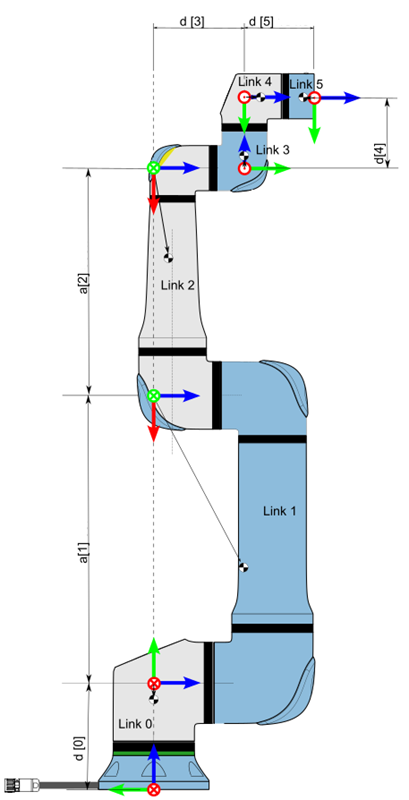
\includegraphics[width=0.3\textwidth]{Static/ur5e_structure.png}
    \caption[UR5eの構成図]{
        UR5eの構成図\cite{ur5e}
    }
    \label{fig:ur5e:structure}
\end{figure}

\begin{table}[htb]
    \centering
    \caption[UR5eのDHパラメータ]{
        UR5eのDHパラメータ\cite{ur5e}
    }
    \label{tab:ur5e:dh}
    \begin{tabular}{ccccc}
        \hline
        \textbf{Joint} & $\bm{\theta}$ [rad] & $\bm{a}$ [m]& $\bm{d}$ [m]& $\bm{\theta}$ [rad]\\
        \hline
        1 & 0 & 0       & 0.1625 & $\pi/2$\\
        2 & 0 & -0.425  & 0       & 0\\
        3 & 0 & -0.3922 & 0       & 0\\
        4 & 0 & 0       & 0.1333 & $\pi/2$\\
        5 & 0 & 0       & 0.0997 & $-\pi/2$\\
        6 & 0 & 0       & 0.0996 & 0\\
        \hline
    \end{tabular}
\end{table}


\subsection{モデルの学習}
モデルによる軌道予測の流れを\figref{fig:model:learning:exp3}に示す.
\begin{figure}[htb]
    \centering
    \includesvg[width=0.5\textwidth, inkscapelatex=false]{Static/chap2_exp3_diagram}
    \caption[モデルによる軌道予測の流れ]{
        モデルによる軌道予測の流れ.
    }
    \label{fig:model:learning:exp3}
\end{figure}
マニピュレータの関節角度の時系列データ$\bm{q}_{t-T \sim t}$を入力, 次の時刻の目標のエンドエフェクタの位置変化量$\bm{dx}_{t}$を出力とするニューラルネットワークを学習する (\eqrefc{eq:model:learning}).
\begin{equation}
    \bm{dx}_{t} = f_{\theta}(\bm{q}_{t-T \sim t}) \label{eq:model:learning}
\end{equation}
ここで, $f_{\theta}$はニューラルネットワーク, $T$は時系列の長さを表す.
目標軌道は$xy$平面における8の字軌道とし, その軌道は\eqrefc{eq:model:target_trajectoryx}, \eqrefc{eq:model:target_trajectoryy}で表される.
\begin{equation}
    x_t=0.25 \sin (\frac{\pi}{5} t) \label{eq:model:target_trajectoryx}
\end{equation}
\begin{equation}
    y_t=0.075 \sin (\frac{2\pi}{5} t) \label{eq:model:target_trajectoryy}
\end{equation}
本実験では1ステップあたりの時間間隔を$0.07$ s, シーケンス全体が$250$ sの軌道を学習に用いた.
また, $z$座標は$z=0.3$ mで固定した.

% 入力
入力であるマニピュレータの関節角度$\bm{q}$は連続値であるため, SNNに入力するために0か1のスパイクに変換する必要がある.
本実験ではスパイク変換のエンコーダとしてThreshold Encodingを用いた.
このエンコーダは, 入力の変化がある閾値$q_{th}$を超えたときに1を出力し, それ以外の場合は0を出力するものである.
ここで, 閾値$q_{th}$を$q_{th}^{max}$から$q_{th}^{min}$までの範囲で$N_{th}$個に分割することで, 入力の変化を$N_{th}$チャンネルのスパイクとして表現することができる.
本実験では入力関節角度は正規化し, $q_{th}^{max}=1.1$, $q_{th}^{min}=-1.1$, $N_{th}=200$とした.

% モデルタイプ
学習させるモデルは通常のSNNおよび提案手法のSNNとした.
それぞれのモデル構成は大きく2つに分けられ, 1つはSNNによる特徴抽出器$f_{\theta}^{SNN}$, もう一つはNNによる予測器$f_{\theta}^{NN}$である.
SNNの出力は0か1のスパイクであるため, 連続値であるエンドエフェクタ座標を直接予測することは困難である.
そこで, 本実験ではSNNを時系列入力の特徴抽出器として扱う.
さらに, SNNの最終層の内部状態$\bm{v}$を特徴量として, 通常のNNで構成された予測器に入力する.
そして, NNによる予測器が教師エンドエフェクタの位置変化量との誤差が小さくなるようにモデルの学習を行う.
ここで, SNNの最終層の内部状態閾値$v_{th}$は無限大とし, 内部状態がリセットされないようにした.
これはSNNのみでVariational Autoencoder (VAE)を構築したFully Spiking VAE (FSVAE)\cite{fsvae}を参考にした構造である.
また, NN予測器の活性化関数はReLU関数とした.
モデルサイズと学習時のパラメータを\tabref{tab:exp3:model:snn} - \tabref{tab:exp3:train:parameter}に示す.
\begin{table}[htb] %\20241112\\eight_figure_shallow3\\snn_beta0.95_seq50",
    \centering
    \caption{マニピュレータ軌道予測モデル : SNN特徴抽出器$f_{\theta}^{SNN}$}
    \label{tab:exp3:model:snn}
    \begin{tabular}{ccc}
        \hline
        \textbf{Input size}& \textbf{Hidden size} & \textbf{Output size}\\
        \hline
        1200   & 512, 128, 64 & 12 \\
        \hline
    \end{tabular}
\end{table}

\begin{table}[htb]
    \centering
    \caption{LIFモデルのパラメータ}
    \label{tab:exp3:model:parameter:lif}
    \begin{tabular}{ccccc}
        \hline
        $\bm{dt}$& $\bm{v_{rest}}$ & $\bm{v_{th}}$ & $\bm{\tau}$ & $\bm{r}$\\
        \hline
        0.03   & 0.0 & 0.1 (最終層のみ$\infty$) & 0.6 & 1 \\
        \hline
    \end{tabular}
\end{table}

\begin{table}[htb] %\20241112\\eight_figure_shallow3\\snn_beta0.95_seq50",
    \centering
    \caption{マニピュレータ軌道予測モデル : NN予測器$f_{\theta}^{NN}$}
    \label{tab:exp3:model:nn}
    \begin{tabular}{ccc}
        \hline
        \textbf{Input size}& \textbf{Hidden size} & \textbf{Output size}\\
        \hline
        12   & 16, 16,16 & 2 \\
        \hline
    \end{tabular}
\end{table}

\begin{table}[htb]
    \centering
    \caption{モデルの学習条件}
    \label{tab:exp3:train:parameter}
    \begin{tabular}{cc}
        \hline
        学習率 $lr$ & 0.001\\
        バッチサイズ $batch\_size$ & 64\\
        エポック数 $epoches$ & 200\\
        勾配クリッピング $clip\_norm$ & 1.0\\
        optimizer & Adam\\
        \hline
    \end{tabular}
\end{table}

学習時の損失関数を\eqrefc{eq:exp3:loss}に示す.
\begin{align}
    \bm{v}^{t,L} &= f_{\theta}^{SNN}(\bm{q}_{t}) \notag \\
    \bm{\hat{dx}}_{t} &= f_{\theta}^{NN}(\bm{v}^{t,L}) \notag \\
    \mathcal{L}_{MSE} &= \frac{1}{T} \sum_{t=1}^{T} \left( \bm{dx}_{t} - \bm{\hat{dx}}_{t} \right)^2 \label{eq:exp3:loss}
\end{align}
ここで, $\bm{v}^{t,L}$は時刻$t$におけるSNNの最終層の内部状態, $\bm{\hat{dx}}^{t}$は時刻$t$における予測器の出力, $\bm{dx}^{t}$は時刻$t$における目標エンドエフェクタの位置変化量である.
また, 損失関数$\mathcal{L}_{MSE}$は入力シーケンスの全ての時刻における予測器の出力と教師データの二乗誤差の平均である.


\subsection{評価方法}
学習済みのモデルを用いて, 軌道速度変化に対するモデル精度評価を行う.
軌道速度変化は\eqrefc{eq:exp3:target_trajectoryx}によって行う.
\begin{equation}
    \bm{x}_{t+1}^{target} = \bm{x}_{t} + \frac{\bm{\hat{dx}}_{t}} {a} \label{eq:exp3:target_trajectoryx}
\end{equation}
ここで, $\bm{x}_{t}$は現在のエンドエフェクタの座標, $\bm{\hat{dx}}_{t}$はモデルの出力, $\bm{x}_{t+1}^{target}$は目標のエンドエフェクタ座標である.
また, $a$は軌道速度変化倍率である.
さらに, 提案手法を用いた軌道予測では, SNNによる特徴抽出器から得られる内部状態$\bm{v_{t,L}}$を速度倍率$a$によってスケーリングする (\eqrefc{eq:exp3:fix:volt}).
\begin{align}
    \bm{{v'}^{t,L}} &= \frac{\bm{v}^{t,L}}{a} \notag \\
    \bm{\hat{dx}}_{t} &= f_{\theta}^{NN}(\bm{{v'}^{t,L}}) \label{eq:exp3:fix:volt}
\end{align}
ここで, $\bm{{v'}^{t,L}}$は速度倍率$a$によってスケーリングされた内部状態である.
連続値入力の速度が$a$倍速に変化したとき, 提案手法およびThreshold Encodingを用いると, SNNの内部状態はタイムスケーリングに加えて, その振幅が$a$倍になる.
そこで, 内部状態$\bm{v}$を速度倍率$a$によってスケーリングし, 理想的な内部状態のタイムスケーリングへ近似する.
速度倍率$a$は0.1, 0.2, 0.3, 0.4, 0.5, 0.6, 0.7, 0.8, 0.9, 1.0, 2.0, 3.0, 4.0, 5.0とした.
それぞれの速度倍率に対して4周期分の軌道の予測および制御を行い, 予測軌道と目標軌道の平均絶対誤差 (Mean Absolute Error, MAE) を評価した.






% 謝辞
\cleardoublepage % 奇数ページから始める
\chapter*{謝辞}
本研究を行うにあたり, 懇切丁寧なる御指導, 御鞭撻を頂きました, 指導教員の林部充宏教授に謹んで深く感謝の意を表します.
研究への取り組み方をはじめ, 勉学以外の面においても, 人として成長するために必要な多くのことを学ばせていただきました.
東北大学大学院情報科学研究科応用情報科学専攻の昆陽雅司教授, 東北大学大学院工学研究科ロボティクス専攻の平田泰久教授, 田村雄介准教授には, 本論文をまとめるにあたって有意義な議論をさせていただきました.
深く感謝いたします.
ミーティングなどにおいて貴重な時間を割いていただき, 本研究を行う過程で数々の有益な御助言をしていただいた大脇大准教授, 沓澤京助教に深く感謝いたします.
研究グループの垣根を越えて議論を交わしていただいた, 同期の田中裕人氏, 反町優平氏, 瀬戸崚生氏, 下山田徹大氏, 横田一樹氏, Laurie Azoulay氏に心より深く感謝いたします.
研究以外の私生活に関する様々な相談に乗っていただき, 大変有意義な二年間を送ることができました.
本研究を行うにあたり様々な面で大変お世話になりました, 研究室の博士, 学部の皆様, 学会での議論に参加していただいた皆様に感謝いたします.
最後になりましたが, これまでの研究生活を温かく見守り, 支えてくれた家族に, この場を借りて心より深く感謝いたします.

\begin{flushright}
2025年2月1日\\
平野 貴也
\end{flushright}



% 参考文献
\printbibliography % 文献リストを出力


\end{document}
% ========================================================================== %